% Options for packages loaded elsewhere
\PassOptionsToPackage{unicode}{hyperref}
\PassOptionsToPackage{hyphens}{url}
\PassOptionsToPackage{dvipsnames,svgnames,x11names}{xcolor}
%
\documentclass[
  12pt,
  a4paper,
  DIV=11,
  numbers=noendperiod]{scrartcl}

\usepackage{amsmath,amssymb}
\usepackage{iftex}
\ifPDFTeX
  \usepackage[T1]{fontenc}
  \usepackage[utf8]{inputenc}
  \usepackage{textcomp} % provide euro and other symbols
\else % if luatex or xetex
  \usepackage{unicode-math}
  \defaultfontfeatures{Scale=MatchLowercase}
  \defaultfontfeatures[\rmfamily]{Ligatures=TeX,Scale=1}
\fi
\usepackage{lmodern}
\ifPDFTeX\else  
    % xetex/luatex font selection
\fi
% Use upquote if available, for straight quotes in verbatim environments
\IfFileExists{upquote.sty}{\usepackage{upquote}}{}
\IfFileExists{microtype.sty}{% use microtype if available
  \usepackage[]{microtype}
  \UseMicrotypeSet[protrusion]{basicmath} % disable protrusion for tt fonts
}{}
\makeatletter
\@ifundefined{KOMAClassName}{% if non-KOMA class
  \IfFileExists{parskip.sty}{%
    \usepackage{parskip}
  }{% else
    \setlength{\parindent}{0pt}
    \setlength{\parskip}{6pt plus 2pt minus 1pt}}
}{% if KOMA class
  \KOMAoptions{parskip=half}}
\makeatother
\usepackage{xcolor}
\usepackage[top=20mm,left=20mm,heightrounded]{geometry}
\setlength{\emergencystretch}{3em} % prevent overfull lines
\setcounter{secnumdepth}{-\maxdimen} % remove section numbering
% Make \paragraph and \subparagraph free-standing
\ifx\paragraph\undefined\else
  \let\oldparagraph\paragraph
  \renewcommand{\paragraph}[1]{\oldparagraph{#1}\mbox{}}
\fi
\ifx\subparagraph\undefined\else
  \let\oldsubparagraph\subparagraph
  \renewcommand{\subparagraph}[1]{\oldsubparagraph{#1}\mbox{}}
\fi

\usepackage{color}
\usepackage{fancyvrb}
\newcommand{\VerbBar}{|}
\newcommand{\VERB}{\Verb[commandchars=\\\{\}]}
\DefineVerbatimEnvironment{Highlighting}{Verbatim}{commandchars=\\\{\}}
% Add ',fontsize=\small' for more characters per line
\usepackage{framed}
\definecolor{shadecolor}{RGB}{241,243,245}
\newenvironment{Shaded}{\begin{snugshade}}{\end{snugshade}}
\newcommand{\AlertTok}[1]{\textcolor[rgb]{0.68,0.00,0.00}{#1}}
\newcommand{\AnnotationTok}[1]{\textcolor[rgb]{0.37,0.37,0.37}{#1}}
\newcommand{\AttributeTok}[1]{\textcolor[rgb]{0.40,0.45,0.13}{#1}}
\newcommand{\BaseNTok}[1]{\textcolor[rgb]{0.68,0.00,0.00}{#1}}
\newcommand{\BuiltInTok}[1]{\textcolor[rgb]{0.00,0.23,0.31}{#1}}
\newcommand{\CharTok}[1]{\textcolor[rgb]{0.13,0.47,0.30}{#1}}
\newcommand{\CommentTok}[1]{\textcolor[rgb]{0.37,0.37,0.37}{#1}}
\newcommand{\CommentVarTok}[1]{\textcolor[rgb]{0.37,0.37,0.37}{\textit{#1}}}
\newcommand{\ConstantTok}[1]{\textcolor[rgb]{0.56,0.35,0.01}{#1}}
\newcommand{\ControlFlowTok}[1]{\textcolor[rgb]{0.00,0.23,0.31}{#1}}
\newcommand{\DataTypeTok}[1]{\textcolor[rgb]{0.68,0.00,0.00}{#1}}
\newcommand{\DecValTok}[1]{\textcolor[rgb]{0.68,0.00,0.00}{#1}}
\newcommand{\DocumentationTok}[1]{\textcolor[rgb]{0.37,0.37,0.37}{\textit{#1}}}
\newcommand{\ErrorTok}[1]{\textcolor[rgb]{0.68,0.00,0.00}{#1}}
\newcommand{\ExtensionTok}[1]{\textcolor[rgb]{0.00,0.23,0.31}{#1}}
\newcommand{\FloatTok}[1]{\textcolor[rgb]{0.68,0.00,0.00}{#1}}
\newcommand{\FunctionTok}[1]{\textcolor[rgb]{0.28,0.35,0.67}{#1}}
\newcommand{\ImportTok}[1]{\textcolor[rgb]{0.00,0.46,0.62}{#1}}
\newcommand{\InformationTok}[1]{\textcolor[rgb]{0.37,0.37,0.37}{#1}}
\newcommand{\KeywordTok}[1]{\textcolor[rgb]{0.00,0.23,0.31}{#1}}
\newcommand{\NormalTok}[1]{\textcolor[rgb]{0.00,0.23,0.31}{#1}}
\newcommand{\OperatorTok}[1]{\textcolor[rgb]{0.37,0.37,0.37}{#1}}
\newcommand{\OtherTok}[1]{\textcolor[rgb]{0.00,0.23,0.31}{#1}}
\newcommand{\PreprocessorTok}[1]{\textcolor[rgb]{0.68,0.00,0.00}{#1}}
\newcommand{\RegionMarkerTok}[1]{\textcolor[rgb]{0.00,0.23,0.31}{#1}}
\newcommand{\SpecialCharTok}[1]{\textcolor[rgb]{0.37,0.37,0.37}{#1}}
\newcommand{\SpecialStringTok}[1]{\textcolor[rgb]{0.13,0.47,0.30}{#1}}
\newcommand{\StringTok}[1]{\textcolor[rgb]{0.13,0.47,0.30}{#1}}
\newcommand{\VariableTok}[1]{\textcolor[rgb]{0.07,0.07,0.07}{#1}}
\newcommand{\VerbatimStringTok}[1]{\textcolor[rgb]{0.13,0.47,0.30}{#1}}
\newcommand{\WarningTok}[1]{\textcolor[rgb]{0.37,0.37,0.37}{\textit{#1}}}

\providecommand{\tightlist}{%
  \setlength{\itemsep}{0pt}\setlength{\parskip}{0pt}}\usepackage{longtable,booktabs,array}
\usepackage{calc} % for calculating minipage widths
% Correct order of tables after \paragraph or \subparagraph
\usepackage{etoolbox}
\makeatletter
\patchcmd\longtable{\par}{\if@noskipsec\mbox{}\fi\par}{}{}
\makeatother
% Allow footnotes in longtable head/foot
\IfFileExists{footnotehyper.sty}{\usepackage{footnotehyper}}{\usepackage{footnote}}
\makesavenoteenv{longtable}
\usepackage{graphicx}
\makeatletter
\def\maxwidth{\ifdim\Gin@nat@width>\linewidth\linewidth\else\Gin@nat@width\fi}
\def\maxheight{\ifdim\Gin@nat@height>\textheight\textheight\else\Gin@nat@height\fi}
\makeatother
% Scale images if necessary, so that they will not overflow the page
% margins by default, and it is still possible to overwrite the defaults
% using explicit options in \includegraphics[width, height, ...]{}
\setkeys{Gin}{width=\maxwidth,height=\maxheight,keepaspectratio}
% Set default figure placement to htbp
\makeatletter
\def\fps@figure{htbp}
\makeatother
% definitions for citeproc citations
\NewDocumentCommand\citeproctext{}{}
\NewDocumentCommand\citeproc{mm}{%
  \begingroup\def\citeproctext{#2}\cite{#1}\endgroup}
\makeatletter
 % allow citations to break across lines
 \let\@cite@ofmt\@firstofone
 % avoid brackets around text for \cite:
 \def\@biblabel#1{}
 \def\@cite#1#2{{#1\if@tempswa , #2\fi}}
\makeatother
\newlength{\cslhangindent}
\setlength{\cslhangindent}{1.5em}
\newlength{\csllabelwidth}
\setlength{\csllabelwidth}{3em}
\newenvironment{CSLReferences}[2] % #1 hanging-indent, #2 entry-spacing
 {\begin{list}{}{%
  \setlength{\itemindent}{0pt}
  \setlength{\leftmargin}{0pt}
  \setlength{\parsep}{0pt}
  % turn on hanging indent if param 1 is 1
  \ifodd #1
   \setlength{\leftmargin}{\cslhangindent}
   \setlength{\itemindent}{-1\cslhangindent}
  \fi
  % set entry spacing
  \setlength{\itemsep}{#2\baselineskip}}}
 {\end{list}}
\usepackage{calc}
\newcommand{\CSLBlock}[1]{\hfill\break\parbox[t]{\linewidth}{\strut\ignorespaces#1\strut}}
\newcommand{\CSLLeftMargin}[1]{\parbox[t]{\csllabelwidth}{\strut#1\strut}}
\newcommand{\CSLRightInline}[1]{\parbox[t]{\linewidth - \csllabelwidth}{\strut#1\strut}}
\newcommand{\CSLIndent}[1]{\hspace{\cslhangindent}#1}

\KOMAoption{captions}{tableheading}
\usepackage{wrapfig}
\usepackage{subcaption}
\usepackage{amsmath}
\usepackage{cancel}
\usepackage{hyperref}
\usepackage{tikz}
\usetikzlibrary{shapes.geometric, arrows, arrows.meta, positioning, calc}
\usepackage{tabularx}
\renewcommand{\maketitle}{}
\usepackage{fancyhdr}
\pagestyle{fancy}
\fancyhf{}
\fancyhead[L]{\rightmark}
\fancyhead[R]{\thepage}
\fancyfoot[C]{\thepage}
\usepackage{colortbl}
\definecolor{cornflowerblue}{RGB}{100,149,237}
\definecolor{darkblue}{RGB}{115,150,255}
\definecolor{lighterblue}{RGB}{131, 191, 212}
\definecolor{lightblue}{RGB}{178,211,220}
\makeatletter
\@ifpackageloaded{caption}{}{\usepackage{caption}}
\AtBeginDocument{%
\ifdefined\contentsname
  \renewcommand*\contentsname{Table of contents}
\else
  \newcommand\contentsname{Table of contents}
\fi
\ifdefined\listfigurename
  \renewcommand*\listfigurename{Figurliste}
\else
  \newcommand\listfigurename{Figurliste}
\fi
\ifdefined\listtablename
  \renewcommand*\listtablename{Tabelliste}
\else
  \newcommand\listtablename{Tabelliste}
\fi
\ifdefined\figurename
  \renewcommand*\figurename{Figur}
\else
  \newcommand\figurename{Figur}
\fi
\ifdefined\tablename
  \renewcommand*\tablename{Tabell}
\else
  \newcommand\tablename{Tabell}
\fi
}
\@ifpackageloaded{float}{}{\usepackage{float}}
\floatstyle{ruled}
\@ifundefined{c@chapter}{\newfloat{codelisting}{h}{lop}}{\newfloat{codelisting}{h}{lop}[chapter]}
\floatname{codelisting}{Listing}
\newcommand*\listoflistings{\listof{codelisting}{List of Listings}}
\makeatother
\makeatletter
\makeatother
\makeatletter
\@ifpackageloaded{caption}{}{\usepackage{caption}}
\@ifpackageloaded{subcaption}{}{\usepackage{subcaption}}
\makeatother
\ifLuaTeX
  \usepackage{selnolig}  % disable illegal ligatures
\fi
\usepackage{bookmark}

\IfFileExists{xurl.sty}{\usepackage{xurl}}{} % add URL line breaks if available
\urlstyle{same} % disable monospaced font for URLs
\hypersetup{
  colorlinks=true,
  linkcolor={blue},
  filecolor={Maroon},
  citecolor={Blue},
  urlcolor={Blue},
  pdfcreator={LaTeX via pandoc}}

\author{}
\date{}

\begin{document}


\newgeometry{left=0cm, right=0cm, top=0cm, bottom=0cm}
\vspace*{0.5cm} 
\hspace*{1.5cm}
\includegraphics[width=10cm]{dokumentobjekter/texstuff/UiT_Logo_Bok_Bla_RGB.png} 


\begin{flushleft}
    \vspace*{0.5cm}
    \hspace*{2.5cm}{\color{black}\fontsize{11}{13.2}\selectfont Handelshøgskolen ved UiT \\[0.2em]
    \hspace*{2.5cm}\color{black}\fontsize{8}{13.2}\selectfont Fakultet for biovitenskap, fiskeri og økonomi \\[0.2em]
    \hspace*{2.5cm}\large{\color{black}\textbf{Mappeoppgave 2}}  \\[0.5em]
    \hspace*{2.5cm}\color{black}\fontsize{12}{14.4}\selectfont Mappeoppgave 2 i: SOK-2030 Næringsøkonomi og konkurransestrategi \\[0.5em]
\hspace*{2.5cm}\color{black}\fontsize{11}{13.2}\selectfont Kandidatnummer: 18 \\[0.5em]
    \hspace*{2.5cm}\color{black}\fontsize{11}{13.2}\selectfont Sok-2030, Vår 2024 \\[0.5em]
    \hspace*{2.0cm}
    \par}
\end{flushleft} 



\begin{tikzpicture}[remember picture, overlay]
    \node[anchor=south west, inner sep=0] at (current page.south west) {
\includegraphics[width=\paperwidth]{dokumentobjekter/texstuff/forside_bilde.png}};
\end{tikzpicture}


\newgeometry{left=20mm, right=20mm, top=20mm, bottom=20mm}





\thispagestyle{plain}
\begin{center}
    \Large
    \textbf{Forord}
\end{center}

I oppgaven så er det ikke fjernet oppgave tekst. Denne teksten er hentet fra oppgavesettet og vil være \textit{markert med kursiv skrift} eller ligge som overskrifter.

Valg av farger i figurer er tatt fra forelesingsslides til forelesing 10 fra figurene under Fusjoner og oppkjøp i dagligvarebransjen  \url{https://uit-sok-2030-v24.github.io/Forelesning%2010%20-%20Horisontale%20fusjoner.pdf}


Vi er blitt fortalt at vi ikke trenger å referere til pensum som forelesingsslides eller boken, så dette er gjort veldig lite. Det er satt inn referanser til boken når jeg har følt at jeg har hentet lite fra forelesingene og heller særdeles mye fra boken. 


Brukte tiden min dårlig og dermed ble det dessverre en del slurv på oppgave 2C så er ikke akkurat fornøyd med den.






\newpage
\hypersetup{linkcolor=black}
\renewcommand{\contentsname}{Innholdsfortegnelse}
\renewcommand*{\figureautorefname}{Figur}
\renewcommand*{\tableautorefname}{Tabell}
\tableofcontents
\listoffigures
\listoftables
\hypersetup{linkcolor=blue}
\newpage

\begin{center}
    \Large
    \textit{1.  Oppgave 1 (30\%)}
\end{center}

\textit{Olivita AS ble etablert i 2002 av to professorer fra Universitetet i Tromsø (UiT). Selskapet tilbyr kosttilskuddet Olivita, som inneholder omega-3 og er utviklet for å støtte hjerte, ledd og immunforsvar. Produktet har vært patentbeskyttet frem til 2023, og Olivita har hatt eksklusiv rett til produksjon av dette omega-3 produktet. Etter patentets utløp har det nye selskapet Dr Choice AS kommet på markedet og tilbyr Easy Choice Omega-3. I markedet for omega-3 produkter vil Olivita AS fortsette å være en ledende aktør, mens Dr Choice AS vil utfordre som en nykommer.}

\textit{I dette marked er det følgende invers etterspørsel}

$$
P = 990 - \frac{1}{60}(q_O + q_C)
$$ 
\textit{hvor} $q_O$ \textit{er antall solgte flasker med Olivita,} $q_C$ \textit{er antall solgte flasker Easy Choice Omega-3 og} $P$ \textit{er pris per flaske av Omega-3 produktene. I produksjon av Omega-3 produktene vil begge bedriftene ha konstante marginalkostnader på kr 50 per produsert flaske. Faste kostnader for begge bedriftene er på 3 millioner kroner.}

\subsection{Optimal tilpasning}\label{optimal-tilpasning}

\subsubsection{a) Hva blir optimal tilpasning i dette markedet når Olivita kan gjøre sine strategiske valg før konkurrenten, Dr Choice AS, gjør sitt valg?}\label{a-hva-blir-optimal-tilpasning-i-dette-markedet-nuxe5r-olivita-kan-gjuxf8re-sine-strategiske-valg-fuxf8r}

For å beregne dette må jeg først bestemme hvilken modell som skal brukes
ut ifra de tre modellene som er brukt i kurset: Cournot, Bertrand eller
Stackelberg. I Cournot og Stackelberg konkurrerer bedriftene på kvantum,
mens i Bertrand konkurrerer de på pris. Valget av modell avhenger av om
produktene er strategiske komplementer eller substitutter. Disse
modellene er oligopolmodeller, som brukes for markeder med få aktører
hvor i Bertrand og Cournot så gjøres valgene simultant mens i
Stackelberg så gjøres valgene sekvensielt.

Strategiske komplimenter betyr for eksempel varer som er komplimenter
til hverandre, som for eksempel kaffe og melk. Hvis prisen på kaffe øker
så vil etterspørselen etter melk også øke. Strategiske substitutter er
varer som er substitutter til hverandre, altså varer som er svært like
hverandre som for eksempel Pepsi og Coca Cola. Hvis prisen på Pepsi øker
så vil etterspørselen etter Coca Cola øke.

Da det er sekvensielle valg og bedriftene har samme kostnader, bruker
jeg Stackelberg-modellen, som modellerer hvordan aktørene tar valg i en
sekvensiell rekkefølge. Stackelberg-modellen analyserer hvilket kvantum
som produseres av hver aktør i et marked når en aktør tar sitt valg
først og den andre aktøren tar sitt valg etterpå.

Grunnen til at jeg bruker en kvantumsmodell er at jeg antar at disse
varene er strategiske substitutter. Dette betyr at hvis en bedrift øker
sin produksjon vil det føre til at konkurransebedriften vil redusere sin
produksjon. Dette vises under
\hyperlink{begrunnelse}{begrunnelsen av valg av modell} på
reaksjonsfunksjonen til bedriftene.

Denne modellen løses i to trinn der lederbedriften, Olivita, velger sitt
kvantum i trinn 1, men modellen løses baklengs ved at vi først løser
trinn 2. Grunnen til dette er at Olivita vil finne ut Dr Choice AS sin
beste reaksjonsfunksjon til enhver mengde Olivita produserer. Dette gjør
at Olivita kan maksimere sin egen profitt ved å velge kvantum som gir
høyest profitt gitt Dr Choice AS sin reaksjon. (Pepall et al., 2014, s.
265-268)

\newpage

\begin{table}[t]
\centering
\begin{tabular}{|c|l|}
\hline
\textbf{Variabel} & \textbf{Forklaring} \\
\hline
$\pi_i$ & Profitt hvor $i$ indikerer hvilken bedrift det tilhører\\
\hline
$I$ & Inntekt, altså pris per vare ganger kvantum solgt \\
\hline
$c_i$ & Marginalkostnad per vare produsert \\
\hline
$f_i$ & Faste kostnader for en gitt bedrift \\
\hline
$P$ & Pris per vare, for en gitt bedrift \\
\hline
$Q$ & Kvantum i markedet som er summen av alle $q_i$ altså $\Sigma q_i$ \\
\hline
$q_i^*$ & Optimalt kvantum produsert av en gitt bedrift \\
\hline
$q_i$ & Kvantum produsert av en gitt bedrift \\
\hline
$a$ & Representerer maksimal betalingsvillighet \\
\hline
$b$ & Koeffisient for prisfølsomhet i markedet \\
\hline
$RF_i$ & Reaksjonsfunksjon for bedrift $i$ \\
\hline
\end{tabular}
\caption{Definisjoner av variabler}
\label{tab:definitions}
\end{table}

I denne tabellen er forklaringen til de forskjellige variablene som vil
brukes i beregningene videre.

Vi setter så opp profittfunksjonene for begge bedriftene ved å ta
markedspris per enhet minus marginalkostnad, multiplisert med kvantum
solgt, minus faste kostnader.

\begin{align*}
\pi_O=(P-50) \cdot q_O-3000000 \\
\pi_C=(P-50) \cdot q_C-3000000
\end{align*}

Begge bedriftene har samme marginalkostnader og faste kostnader så jeg
skriver disse som en felles profitt funksjon. Jeg gjør det også på
generell form da utregningene kan bli rotete.

Den inverse etterspørselen er da gitt ved: \[
P = a - b(Q)
\] For å tilpasse denne modellen til Stackelberg-konkurranse, der
Olivita gjør sitt valg først, bruker vi følgende profittfunksjon for
Olivita:

\[
\pi_O = q_O \cdot (a - b \cdot (q_O + q_C) - c) 
\] Jeg løser så trinn 2 først ved å derivere profitten til Dr Choice AS
med hensyn på \(q_C\) og får:

\[
\frac{\partial \pi}{\partial q_C} = a- 2bq_C - bq_O -c
\]

Når denne nå settes lik null får jeg reaksjonsfunksjonen til Dr Choice
AS.

\[
RF_C = q_C= \frac{a-bq_O - c}{2b}
\]

Denne settes så inn i for \(q_C\) i den deriverte profittfunksjonen til
Olivita og løses for \(q_O\) for Trinn 1 i Stackelberg-modellen.

\[
q_O = a-\frac{b q_O}{2} - b \left(q_O + \frac{2-b q_O - c}{2b}\right)-c
\]

\paragraph{Optimalt kvantum}\label{optimalt-kvantum}

Denne løses for \(Q_O\) for å finne optimalt kvantum for Olivita som
velger sitt kvantum først. \[
RF_O = q_O^* = \frac{a-c}{2b}
\]

Vi setter \(RF_O\) så inn i reaksjonsfunksjonen til Dr Choice AS for å
finne optimalt kvantum for Dr Choice AS.

\[
q_C^* = \frac{\frac{a}{2}-\frac{c}{2}}{2b} = \frac{a-c}{4b}
\]

Da \(Q\) = \(Q_O + Q_C\) så kan vi finne prisen i markedet.

\begin{align*}
P &= a - b(q_O + q_C) \\
&= a- b \left(\frac{a-c}{2b} + \frac{a- bq_O - c}{2b} \right) \\
&= \frac{3b q_O}{2} + c
\end{align*}

Ved å sette inn tall for variablene og bruker den opprinnelige
etterspørselsfunksjonen så får vi:

\begin{verbatim}
Kvantum for Olivitas: 28200 og Kvantum for Dr Choice AS: 14100. 
Det totale kvantumet i markedet er 42300 til en Markedsprisen på 285.

Profitten for selskapene er 3627000 for Olivitas og 313500 for Dr Choice AS.
\end{verbatim}

\begin{figure}[h]
\centering
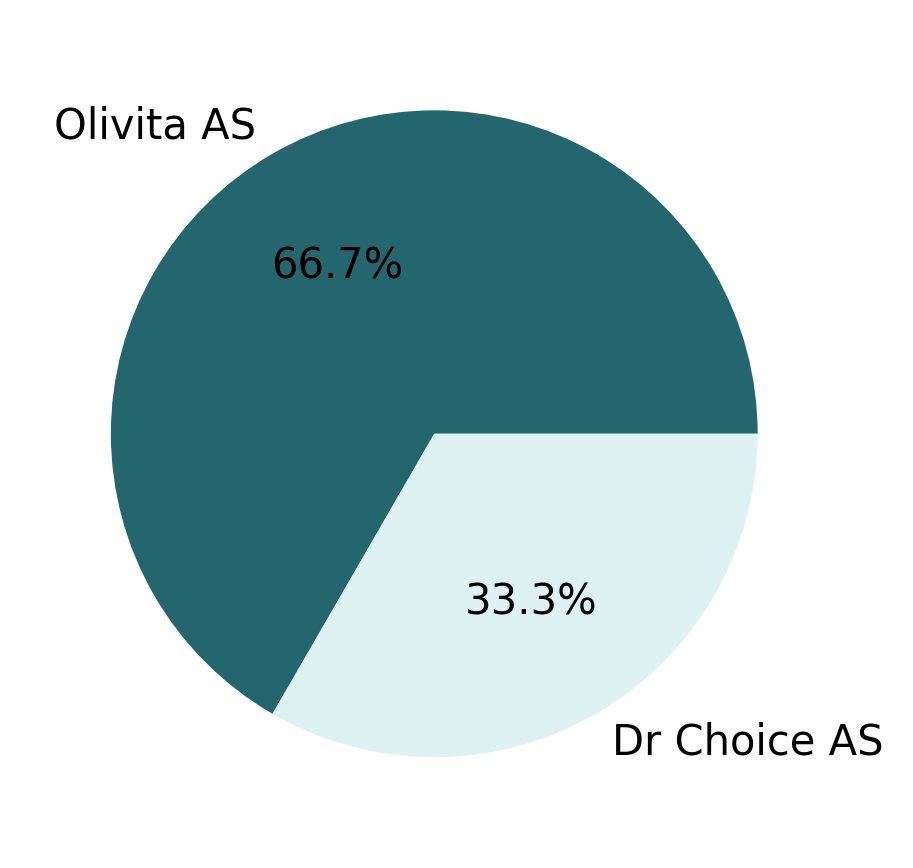
\includegraphics[width=0.9\textwidth]{dokumentobjekter/figurer/markedsandel_stackelberg.png}
\caption{Markedsandelen til Omega-3 produsentene i Stackelberg-modellen.}
\label{fig:markedsandel_oppgave1_a}
\end{figure}

\newpage

\subsubsection{b) Vil det være en fordel for Olivita å ha mulighet til å
gjøre sine valg før konkurrenten gjør sitt
valg?}\label{b-vil-det-vuxe6re-en-fordel-for-olivita-uxe5-ha-mulighet-til-uxe5-gjuxf8re-sine-valg-fuxf8r-konkurrenten-gjuxf8r-sitt-valg}

Som vi kan se i \autoref{fig:markedsandel_oppgave1_a} vil det være en
fordel for Olivita å gjøre sine strategiske valg først. For å bekrefte
dette så vil jeg beregne hvilket kvantum de ville valgt i en vanlig
Cournot-modell uten sekvensiell valg.

\paragraph{Cournot-modell}\label{cournot-modell}

Jeg gjøre dette igjen på generell form for å så sette inn tall og
starter med den inverse etterspørselsfunksjonen. \[
P = a - b(q_O + q_C)
\] Marginalkostnaden til begge bedriftene er konstant og lik og for å
finne etterspørselsfunksjonen for hver bedrift betraktes produsert
mengde for den andre bedrift som konstant.

Etterspørselen til Dr Choice AS er gitt ved: \[
P_C = (a  + bq_O)-bq_C
\] For å finne optimalt kvantum for Dr Choice AS så derivertes
profittfunksjonen til Dr Choice AS med hensyn på \(q_C\) for å finne
marginalinnekten.

\begin{align*}
\pi_C = (P_C - c)q_C = (a  + bq_O - bq_C - c)q_C \\
\frac{\pi_C}{\partial q_C} = (a - bq_O) - 2bq_C
\end{align*}

Dette gir oss optimalt kvantum for Dr Choice AS ved å sette lik marginal
kostnad. \[
q_C = \frac{a - c}{2b} - \frac{q_O}{2}
\]

Vi kan så finne reaksjonsfunksjonen til Olivita ved å sette dette
kvantumet inn i etterspørselen til Olivita. \[
RF_Q = q_O = \frac{a - c}{2b} - \frac{q_C}{2}
\] Vi løser denne ved å sette inn for \(q_C\) \[
q_O = \frac{a - c}{2b} - \left(\frac{\frac{a - c}{2b} - \frac{q_O}{2}}{2}\right)
\] Som endelig gir oss \[
q_O^* = \frac{a - c}{3b} = q_C^*
\]

Vi kan nå finne markedsprisen ved å sette inn kvantum for begge
bedriftene i den inverse etterspørselen.

\begin{verbatim}
Kvantum for Olivitas: 18800 og kvantum for Dr Choice AS blir 18800. 
Det totale kvantumet i markedet er 42300 til en Markedsprisen på 363.

Profitten for selskapene er 2060363 for Olivitas og 2060363 for Dr Choice AS.
\end{verbatim}

Så vi kan se at dersom Olivita ikke får gjøre sitt valg først så vil det
totale kvantumet i markedet være på bare 37600 enheter som er lavere enn
det totale kvantumet under Stackelberg på 42300. Dette viser oss også at
de får like markedsandeler.

Det er også en høyere pris på 363 istedet for 285. Profitten til Olivita
har også sunket fra 3 627 000 til 2 060 363 så ja det er en fordel for
Olivita å gjøre sine valg først.

\subsubsection{Begrunnelse for valg av
modell}\label{begrunnelse-for-valg-av-modell}

$\displaystyle 28200.0 - 0.5 Q_{C}$

$\displaystyle 28200.0 - 0.5 Q_{O}$

\hypertarget{begrunnelse}{Her har jeg tatt å satt inn for verdiene til}

\(a\), \(b\) og \(c\) i reaksjonsfunksjonene til bedriftene. Det vi kan
se er at begge reaksjonsfunksjonene har negativ helning så dersom
Olivita øker sin produksjon så vil reaksjonsfunksjonen til Dr Choice AS
reduseres og det samme vil skje dersom Dr Choice AS øker sin produksjon.
Dette tyder på at det er strategiske substitutter.

I Cournot-modellen oppnår vi en Nash-likevekt der ingen av bedriftene
kan øke sin profitt ved å ensidig endre sitt produksjonskvantum.
Likevekten i Stackelberg-modellen gir Olivita en fordel ved at de kan
utnytte sin lederposisjon til å påvirke markedsforholdene til sin
fordel, noe som resulterer i høyere totalproduksjon og lavere
markedspris. Nash likevekt er en tilstand i et spill der bedriftene ikke
jobber sammen og derfor ikke kan oppnå en bedre posisjon ved å endre
strategi gitt at de andre bedriftene holder seg til sin strategi. Som vi
kan se så har Olivitas og Dr Choice oppnådd en Nash-likevekt når de har
basert seg på hva de tror den andre bedriften vil produsere. De er nå
fornøyd med sin produksjon og har ingen insentiver til å endre den.

I Stackelberg-modellen der en bedrift kan ta et valg først og deretter
den andre bedriften kan ta sitt valg så kan Olivitas som velger først
utnytte sin posisjon og dermed oppnå en høyere profitt enn i
Cournot-modellen. Dette er fordi Olivitas kan øke sin produksjon og
dermed redusere produksjonen til Dr Choice AS som vil føre til en høyere
markedspris og dermed en høyere profitt for Olivitas. Dette er en fordel
for Olivitas og en ulempe for Dr Choice AS.

\clearpage

\subsection{Optimal tilpasning før
fusjon}\label{optimal-tilpasning-fuxf8r-fusjon}

\begin{center}
    \Large
    \textit{2.  Oppgave 2 (70\%)}
\end{center}

\textit{Markedet for produksjon av mikroøl består av tre lokale bryggerier: Graff Brygghus, Bryggeri 13 og Mack Mikrobryggeri. Etterspørselen i dette markedet er gitt ved:} 
$$
P = 175-4Q
$$ 
\textit{hvor }$P$ \textit{er markedspris per flaske mikroøl,} $Q$ \textit{er totalt kvantum (antall tusen flasker), som er summen av produksjonen til de tre bryggeriene: }$Q = q_G + q_B + q_M$, \textit{der }$q_G$ \textit{er produsert kvantum for Graff Brygghus,} $q_B$ \textit{er produsert kvantum for Bryggeri 13 og} $q_M$ \textit{er produsert kvantum for Mack Mikrobryggeri.}

\textit{Mack Mikrobryggeri, som er en del av Mack Ølbryggeri, har en mer effektiv produksjonslinje enn de to andre, med konstante marginalkostnader på 7 kr per flaske, mens Graff Brygghus og Bryggeri 13 har marginalkostnader på 10 kr per flaske. Alle tre mikrobryggeriene har faste årlige kostnader på 300 000 kr. Styrene i selskapene Mack Mikrobryggeri og Bryggeri 13 har startet samtaler knyttet til mulig fusjon av disse to selskapene. Ved en fusjon vil all produksjon flyttes til Mack Mikrobryggeri. De faste kostnadene vil også reduseres ved sammenslåing av selskapene, og totalt utgjøre kr 500 000 per år for det fusjonerte selskapet.}

\subsubsection{a) Vil en slik fusjon være lønnsom for de fusjonerte
partene?}\label{a-vil-en-slik-fusjon-vuxe6re-luxf8nnsom-for-de-fusjonerte-partene}

I en slik situasjon så starter jeg med å beregne hvordan markedet er før
en fusjon ved bruk av Cournot-modellen for bedrifter med asymmetriske
bedrifter siden en av de tre bedriftene har forskjellige kostnader. Da
varene er homogene eller veldig like, så antar vi at det er samme
kundebase for alle tre og at bedriftene konkurrerer med kvantitet.

\paragraph{Cournot modellen før
fusjon}\label{cournot-modellen-fuxf8r-fusjon}

For å finne likevekten i markedet før fusjon så starter vi med å finne
reaksjonsfunksjonene til bedriftene. Jeg viser dette igjen på generell
form for å gjøre det ryddigere og lettere å forstå.

Jeg skriver da igjen etterspørselsfunksjonen som: \[
P = a - bQ
\] \(Q\) er igjen lik \(\Sigma q_i\) og vi har at
\(Q = q_G + q_B + q_M\). der \(q_G\) er for Graff Brygghus, \(q_B\) er
for Bryggeri 13 og \(q_M\) er for Mack Mikrobryggeri. Inntektene til
bedriftene er gitt ved \(I\): \[
I_i = P \cdot q_i\cdot(a-b\cdot q_i)
\] og kostnader er gitt ved: \[
c_i = q_i \cdot c_i + f_i
\]

Dette kan settes sammen for å gi oss profittfunksjonen til bedriftene:

\begin{align*}
\pi_G &= -c_G\cdot q_G - f_G + (a-b\cdot(q_G+q_B+q_M))\cdot q_G \\
\pi_B &= -c_B\cdot q_B - f_B + (a-b\cdot(q_G+q_B+q_M))\cdot q_B \\
\pi_M &= -c_M\cdot q_M - f_M + (a-b\cdot(q_G+q_B+q_M))\cdot q_M
\end{align*}

Jeg deriverer så disse og løser for \(q_i\) for å finne
reaksjonsfunksjonene til bedriftene og setter inn verdier for \(a\),
\(b\) og \(c_i\) for å finne kvantumene som produseres av bedriftene.

\begin{align*}
q_B &= \frac{a-3\cdot c_B + c_G + c_M}{4\cdot b}= \frac{175-3\cdot 10 + 10 + 7}{4\cdot 4} = 10.125 \\
q_G &= \frac{a + c_B - 3\cdot c_G + c_M}{4\cdot b} =  \frac{175 + 10 - 3\cdot 10 + 7}{4\cdot 4} = 10.125 \\
q_M &= \frac{a + c_B + c_G -3\cdot c_M}{4\cdot b} = \frac{175 + 10 + 10 -3\cdot 7}{4\cdot 4} = 10.875
\end{align*}

Tallene er oppgitt i tusener som gir oss at Graff Brygghus og Bryggeri
13 produserer 10125 flasker mikroøl, mens Mack Mikrobryggeri produserer
10875 flasker mikroøl.

\begin{figure}[h]
\centering
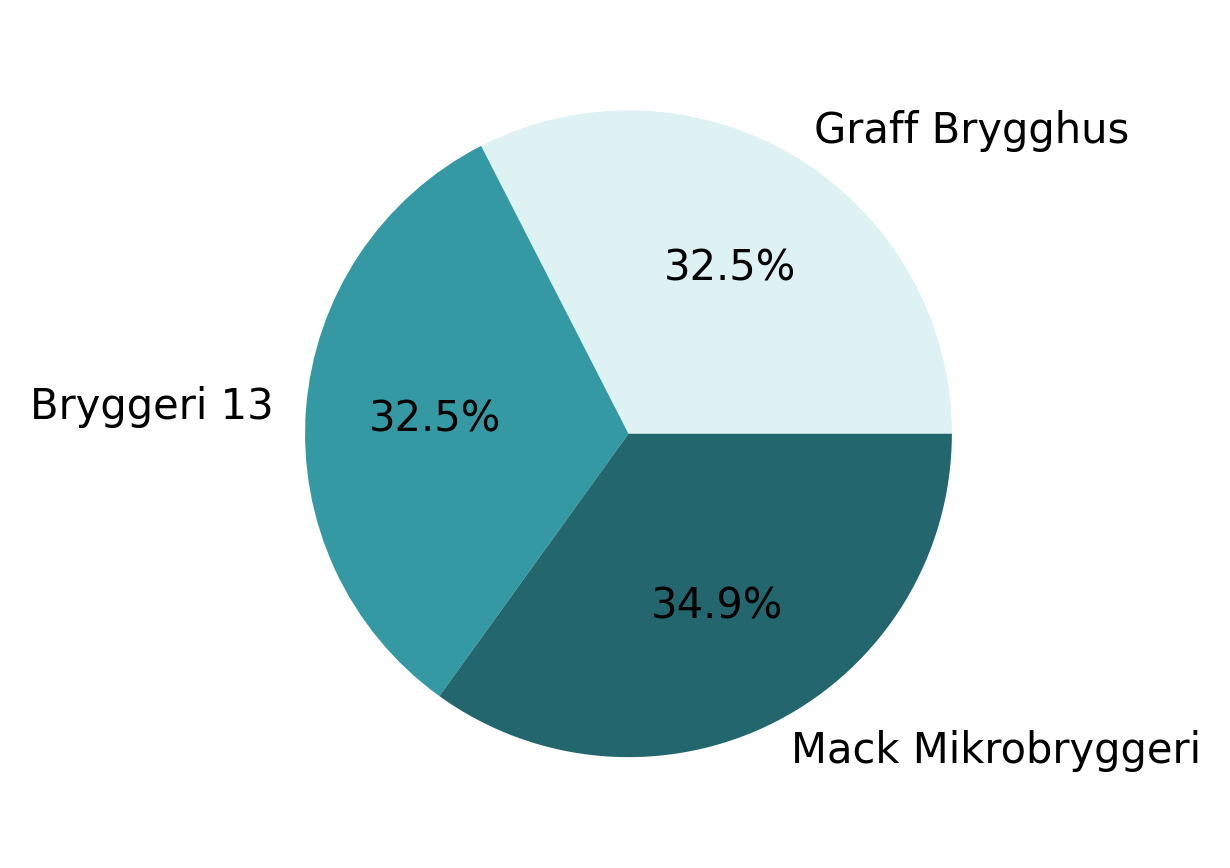
\includegraphics[width=0.9\textwidth]{dokumentobjekter/figurer/markedsandel_mikrobryggerier.png}
\caption{Markedsandelen til mikrobryggeriene}
\label{fig:markedsandel}
\end{figure}

For å nå finne markedsprisen så setter jeg dette inn i
etterspørselsfunksjonen og får: \[
P = 175 - 4\cdot(10.125 + 10.125 + 10.875) = 175 - 4\cdot 31.125 = 175 - 124.5 = 50.5
\] Dette gir oss at markedsprisen er 50.5 kr per flaske mikroøl. Så kan
jeg bare sette inn tallene i de tidligere profittfunksjonene og får:

\begin{align*}
\pi_G = 110.0625 \\
\pi_B = 110.0625 \\
\pi_M = 173.0625
\end{align*}

Da tallene er gitt i tusen så gir dette oss at Graff Brygghus og
Bryggeri 13 hadde hver en profitt på 110 062.5kr, mens Mack
Mikrobryggeri har en profitt på 173 062.5kr.

Nå starter jeg ved å se på hva som skjer om Mack Mikrobryggeri og
Bryggeri 13 fusjonerer.

\clearpage

\subsection{Optimal tilpasning etter
fusjon}\label{optimal-tilpasning-etter-fusjon}

Når Mack Mikrobryggeri og Bryggeri 13 fusjonerer vil vi ha et marked med
2 aktører med asymmetriske kostnader. Derfor bruker jeg igjen
Cournot-modellen for asymmetriske bedrifter men nå med 2 aktører. Jeg
blir å betegne Mack og Bryggeri 13 \(BM\). Jeg setter opp ligningene for
profitten til hver av bedriftene etter fusjonen:

\begin{align*}
\pi_G = -cG \cdot q_G + f_G + q_G \cdot (a - b \cdot (q_G + q_{BM}))\\
\pi_BM = -c_{BM} \cdot q_{BM} - f_{BM} + q_{BM} \cdot (a - b \cdot (q_G + q_{BM}))
\end{align*}

Jeg deriverer disse og løser for \(q_G\) og \(q_{BM}\) for å finne
reaksjonsfunksjonene og kvantum:

\begin{align*}
q_G = \frac{a-2\cdot c_G + c_{BM}}{3\cdot b} = \frac{175-2\cdot 10 + 7}{3\cdot 4} =  13.5\\
q_{BM} = \frac{a + c_G -2\cdot c_{BM}}{3\cdot b} = \frac{175 + 10 -2\cdot 7}{3\cdot 4} = 14.25
\end{align*}

Ved å substituere inn tallene får vi at Mack Mikrobryggeri vil produsere
13500 flasker mikroøl, mens Bryggeri 13 vil produsere 14250 flasker
mikroøl.

Jeg kan nå sette dette inn i etterspørselsfunksjonen å få markedspris \[
p = 175 - 4 \cdot (13.5 + 14.25) = 64
\]

Vi ser at denne prisen er høyere enn den opprinnelige prisen før fusjon.
Jeg kan nå sette dette inn i profittfunksjonene for å finne profitten i
tusener til hver av bedriftene etter fusjonen.

\begin{align*}
\pi_G = 429 \\
\pi_{BM} = 312.25
\end{align*}

Vi ser at Graff Brygghus har tjent mer på fusjonen enn de fusjonerte
selskapene Mack og Bryggeri 13. Vi kan også se hvordan markedsandelene
har endret seg i \autoref{fig:markedsandel_etter}.

\begin{figure}[t]
\centering
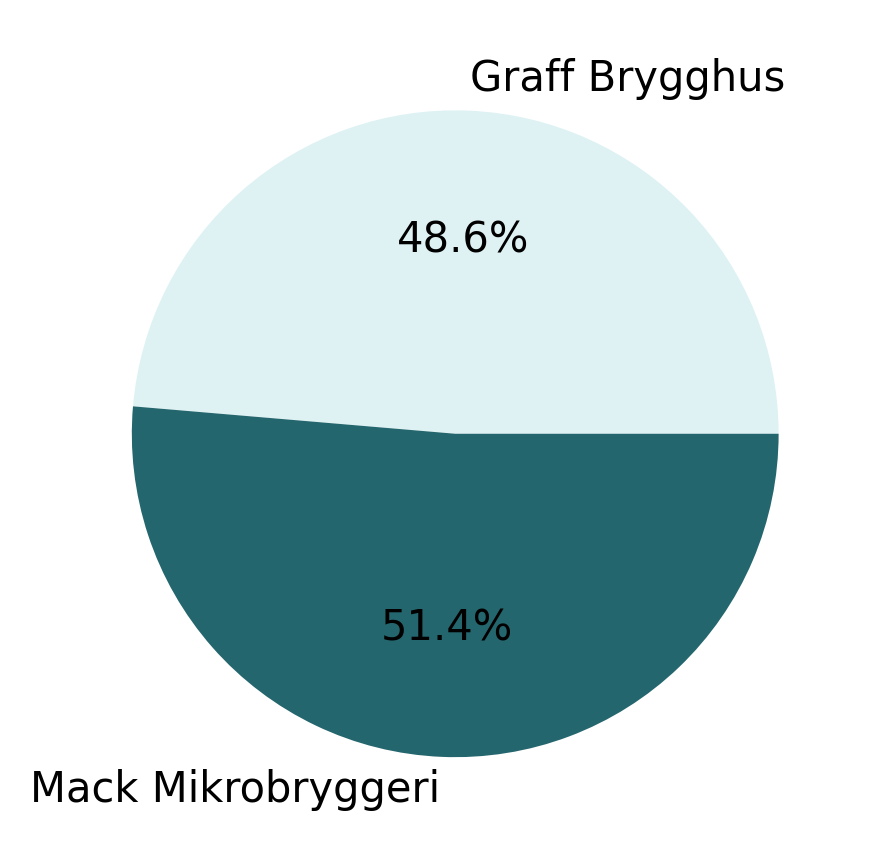
\includegraphics[width=0.7\textwidth]{dokumentobjekter/figurer/markedsandel_mikrobryggerier_fusjon.png}
\caption{Markedsandelen til mikrobryggeriene etter fusjonen}
\label{fig:markedsandel_etter}
\end{figure}

Paradoksialt nok så kan vi se at fusjonen mellom Mack Mikrobryggeri og
Bryggeri 13 har resultert i økt profitt for Graff Brygghus, som ikke er
en del av fusjonen. Dette skjer fordi fusjonen mellom de to
konkurrentene reduserer konkurransen i markedet. Når Mack Mikrobryggeri
og Bryggeri 13 fusjonerer, blir de mer effektive sammen, og de totale
produksjonskostnadene deres reduseres. Men som vi ser så vil dette føre
til en samlet reduksjon i markedets tilbud, noe som igjen øker
markedsprisen. Graff Brygghus som fortsatt opererer uavhengig, kan nå
dra nytte av høyere priser i markedet uten å endre sine egne kostnader
eller produksjonsnivå.

\paragraph{Økt Profitt for
bedriftene}\label{uxf8kt-profitt-for-bedriftene}

Graff Brygghus vil øke sitt produksjonskvantum fra 10125 flasker til
13500 flasker etter fusjonen. Denne økningen i produksjon kombinert med
en 13.5kr økning i markedspris per flaske resulterer i en betydelig
økning i Graff Brygghus sin profitt. Før fusjonen var profitten deres
110 062.5kr og etter fusjonen vil profitten øke til 429 000kr.

Men selv om Graff Brygghus har hatt en stor økning i profitt, vil også
det fusjonerte selskapet Mack Mikrobryggeri og Bryggeri 13 få en høyere
profitt. Før fusjonen var deres samlede profitt 173 062.5kr for Mack og
110 062.5kr for Bryggeri 13, noe som tilsammen utgjør 283 125kr. Etter
fusjonen vil de ha en profitt på 312 250kr. De produserer nå mindre enn
de ville gjort samlet fra samlet 21000 flasker til 14250 flasker etter.

Så fusjonen vil gi økt profitt for begge bedriftene. Selv om det har
vært bedre for Graff Brygghus, vil Mack og Bryggeri 13 også tjene mer på
fusjonen gjennom økte priser. Av den grunn vil fusjonen være en god ide
for begge bedriftene.

\paragraph{Forklaring av Fusjonsparadokset symmetriske bedrifter
generelt}\label{forklaring-av-fusjonsparadokset-symmetriske-bedrifter-generelt}

Fusjonsparadokset er det uintuitive som skjer i horisontale fusjoner i
Cournot-modellen hvor det viser seg at det ikke vil være lønnsomt for de
fusjonerende selskapene, men lønnsomme for de ikke-fusjonerende
selskapene. Bedriftene konkurrerer i kvantitet som fører en fusjon
mellom to selskaper i et tre-selskapsmarked til at de fusjonerte
selskapene oppnår lavere samlet produksjon og lavere samlet profitt enn
før fusjonen. Dette er fordi antallet aktører i markedet reduseres, noe
som øker markedsprisen. Denne prisøkningen er til fordel for det
ikke-fusjonerte selskapet, som kan øke sin produksjon og selge til en
høyere pris. De fusjonerte selskapene, derimot, produserer nå samlet
sett mindre enn de gjorde individuelt før fusjonen, og dermed reduseres
deres samlede profitt.(Pepall et al., 2014, s. 388-394)

\newpage

\paragraph{Kostnadssynergier i asymmetriske bedrifter i
casen}\label{kostnadssynergier-i-asymmetriske-bedrifter-i-casen}

I dette tilfellet ser vi at Graff Brygghus drar nytte av fusjonen mellom
Mack Mikrobryggeri og Bryggeri 13 ved å kunne selge sitt økte kvantum
til en høyere pris. Samtidig har det fusjonerte selskapet oppnådd
kostnadssynergier som gir dem en økning i effektiviteten og en økt
samlet profitt enn før fusjonen på grunn av økt markedspris. Men i
virkeligheten så er det ikke bare en gang du velger kapasitet og med
denne økte kapasiteten og lavere marginale kostnader med lavere faste
kostnader enn hver for seg vil det fusjonerte selskapet kunne innta en
lederposisjon i markedet og dermed endre dynamikken i markedet. Dette
vil føre til at det fusjonerte selskapet vil ha en fordel i markedet og
at det er Stackelberg-modellen som bør brukes.

\paragraph{Stackelberg-modellen}\label{stackelberg-modellen}

En fusjon mellom Mack Mikrobryggeri og Bryggeri 13 der kapasiteten
flyttes over til mack vil da gi dobbel kapasitet med den lavere
marginalkostnaden og lavere faste kostnader enn de hadde individuelt.
Dermed vil en fusjon føre til at det fusjonerte selskapet vil ha en
fordel i markedet slik at de vil innta en leder posisjon i markedet.
Derfor er det Stackelberg-modellen som bør brukes.

For å beregne denne så følger jeg samme fremgangsmåte som i oppgave 1a
men med asymmetriske bedrifter. Jeg blir ikke å vise all utregning for å
spare plass men dette gjøres i python. Svarene vises i \autoref{table:3}

\begin{verbatim}
Kvantum for fusjonert Mack: 21.38 og Kvantum for Graff Brygghus: 9.94. 
Det totale kvantumet i markedet er 31.31 til en Markedsprisen på 49.75.

Profitten for selskapene er 413.78 for fusjonert Mack og 95.02 for Graff Brygghus.
\end{verbatim}

\begin{figure}[!h]
\centering
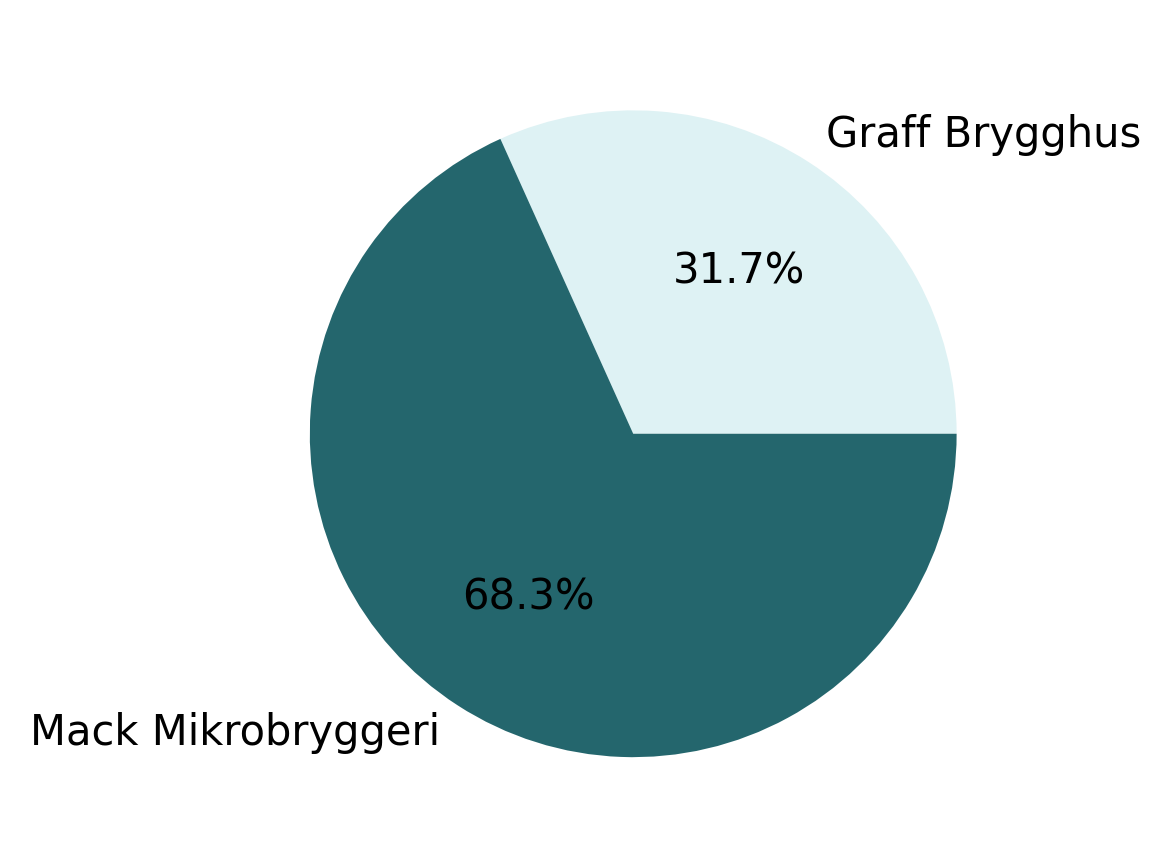
\includegraphics[width=0.7\textwidth]{dokumentobjekter/figurer/markedsandel_mikrobryggerier_fusjon_stackel.png}
\caption{Markedsandelen til mikrobryggeriene etter fusjonen under Stackelberg med ledende Mack}
\label{fig:markedsandel_etter_stackel}
\end{figure}

\clearpage

\begin{table}[h]
\centering
\begin{tabular}{|l|l|l|l|}
\hline
\rowcolor{cornflowerblue} \textbf{Bedrift} & \textbf{Variabel} & \textbf{Cournot} & \textbf{Stackelberg} \\ \hline
\rowcolor{lighterblue} Mack Mikrobryggeri      & Profitt                  & $173060.0~kr$             & -           \\ \hline
\rowcolor{lighterblue} Bryggeri 13  & Profitt                  & $110060.0~kr$             & -           \\ \hline
\rowcolor{lighterblue} Graff Brygghus  & Profitt                  & $110060.0~kr$             & -           \\ \hline 
\textbf{Total}  & -                  & $393180.0~kr$             & -           \\ \hline
\rowcolor{lightblue} Mack Mikrobryggeri      & Kvantum                  & $10875.0$             & -           \\ \hline
\rowcolor{lightblue} Bryggeri 13  & Kvantum                  & $10125.0$             & -           \\ \hline
\rowcolor{lightblue} Graff Brygghus  & Kvantum                  & $10125.0$             & -           \\ \hline 
\textbf{Total}  & -                  & $31125.0$             & -          \\ \hline
- & \textbf{Markedspris} & $50.50~kr$ & - \\ \hline
\rowcolor{cornflowerblue} \textbf{Bedrift etter fusjon} & \textbf{Variabel} & \textbf{Cournot} & \textbf{Stackelberg} \\ \hline
\rowcolor{lighterblue} Fusjonert Mack og Bryggeri      & Profitt                  & $312250.0~kr$             & $413781.25~kr$           \\ \hline
\rowcolor{lighterblue} Graff Brygghus  & Profitt                  & $429000.0~kr$             & $95015.62~kr$           \\ \hline 
\textbf{Total}  & -                  & $741250.0~kr$             & $508796.88~kr$           \\ \hline
\rowcolor{lightblue} Fusjonert Mack og Bryggeri      & Kvantum                  & $14250.0$             & $21375$           \\ \hline
\rowcolor{lightblue} Graff Brygghus  & Kvantum                  & $13500.0$             & $9937.50$           \\ \hline
\textbf{Total}  & -                  & $27750.0$             & $31312.50$           \\ \hline
- & \textbf{Markedspris} & $64.0~kr$ & $49.75~kr$ \\ \hline
\end{tabular}
\caption{Effekten av fusjon mellom Mack og Bryggeri 13}
\label{table:3}
\end{table}

I \autoref{fig:markedsandel_etter_stackel} ser vi at å bruke
Stackelberg-modellen ser ut til å løse fusjonsparadokset og at Mack
Mikrobryggeri vil innta en ledende posisjon i markedet. Dette vil gi en
økt profitt for de fusjonerte selskapene. Det vil også gi en økt profitt
for de fusjonerte selskapene og dette ville gitt en \textbf{lavere
markedspris og totalt høyere kvantum} i markedet. Vi kan uansett
konkludere med at en fusjon mellom Mack Mikrobryggeri og Bryggeri 13 vil
være lønnsomt for de to selskapene.

\clearpage

\textit{Videre i oppgaven skal vi anta at fusjon mellom Mack Mikrobryggeri og Bryggeri 13 blir gjennomført, og det nye selskapet vil operere under navnet Mack Mikrobrygg 13. Markedet for produksjon av mikroøl vil da bestå av to lokale produsenter: Mack Mikrobrygg 13 og Graff Brygghus. For å styrke sin posisjon i markedet, investerer Graff Brygghus i nytt og mer effektivt produksjonsutstyr, noe som reduserer deres variable kostnader til kr 7 per flaske. Denne investeringen vil gi selskapet økte faste kostnader på kr 200.000. Totale faste kostnader for begge bryggeriene er da på kr 500.000 for hvert av selskapene.}

\textit{I restaurantbransjen i Tromsø er Restaurant Gruppen Holdig (RGH) en sentral aktør, som har monopol i sitt segment. RGH kjøper sitt mikroøl fra de to lokale produsentene Mack Mikrobrygg 13 og Graff Brygghus. For å drifte sine restauranter har RGH faste kostnader på kr 600.000.}

\textit{Etterspørselen etter mikroøl i restaurantbransjen er lik:} 
$$
P = 175 - 2Q
$$ 
\textit{hvor }$Q$\textit{ er antall solgte flasker mikroøl (antall tusen flasker) for RGH og }$P$\textit{ er prisen for en flaske mikroøl til sluttbruker. For å ytterligere styrke sin posisjon i oppstrømsmarkedet, vurderer ledelsen i Mack Mikrobrygg 13 en fusjon med konkurrenten Graff Brygghus. Det antas at denne fusjonen ikke vil resultere i kostnadsbesparelser for bryggeriene. Som konsulent for styret i Mack Mikrobrygg 13, er du bedt om å analysere markedskonsekvensene av en potensiell fusjon mellom Mack Mikrobrygg 13 og Graff Brygghus. Analysen skal omfatte en vurdering av dagens markedstilpasning og en sammenligning med tilpasningen etter en eventuell fusjon i oppstrømsmarkedet.}

\subsection{Vertikale relasjoner}\label{vertikale-relasjoner}

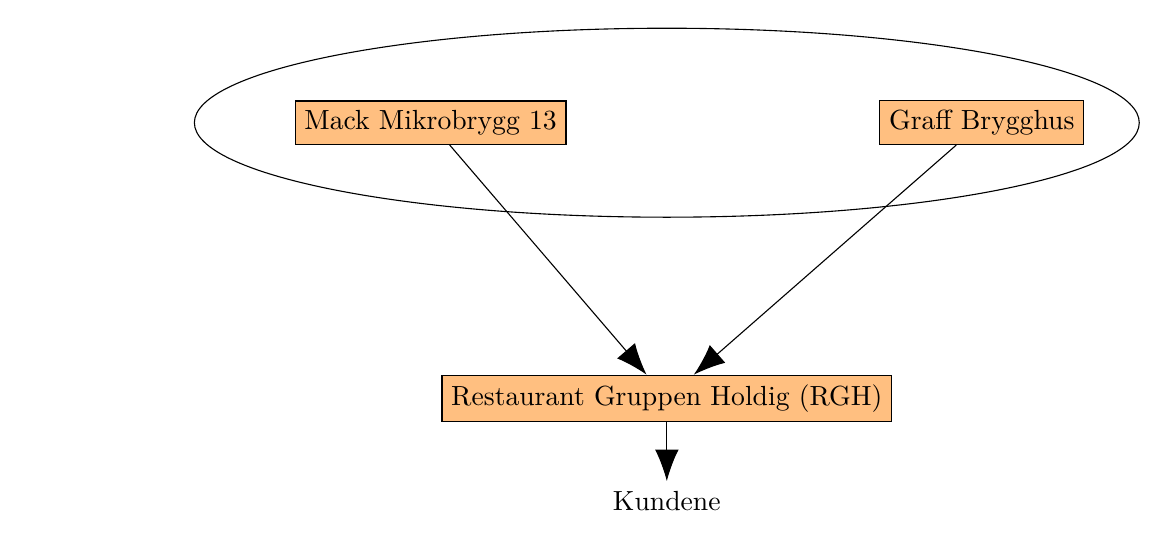
\begin{tikzpicture}[node distance=2cm]
\node (del1) {};

\node (startpunkt)[rectangle, fill=orange!50, draw=black, text centered, right of = del1, xshift=3cm, yshift=5cm] {Mack Mikrobrygg 13};

\node (G)[rectangle, fill=orange!50, draw=black, right of = startpunkt, text centered, xshift=5cm] {Graff Brygghus};
\node (RHG)[rectangle, fill=orange!50, draw=black, below of = startpunkt, text centered, xshift=3cm, yshift=-1.5cm] {Restaurant Gruppen Holdig (RGH)};

\node (Kundene)[below of = RHG, text centered, yshift=0.7cm] {Kundene};



\draw[-{Latex[length=4mm]}] (startpunkt) -- (RHG);
\draw[-{Latex[length=4mm]}] (G) -- (RHG);
\draw[-{Latex[length=4mm]}] (RHG) -- (Kundene);


\fill[fill=none, xshift=5.5cm, yshift=5cm, draw=black] (2.5,0) ellipse (6 and 1.2);

\end{tikzpicture}

I figuren over så kan vi se hvordan markedet ser ut før det gjøres noe
endringer. Mack og Graff er såkalte ``Oppstrømsbedrifter'' som betyr at
de er lengere unna kunden og selger dette til nedstrømsbedriften RGH som
vil selge dette videre til kundene. I dette tilfellet er da Mack og
Graff produsenter i forsyningskjeden til RGH som selger dette videre til
kundene.

Sirkelen rundt Mack og Graff viser hvilke selskap som vil fusjonere.

\clearpage

\subsubsection{b) Basert på din analyse, vil du anbefale styret i Mack
Mikrobrygg 13 å gjennomføre fusjon med Graff
Brygghus?}\label{b-basert-puxe5-din-analyse-vil-du-anbefale-styret-i-mack-mikrobrygg-13-uxe5-gjennomfuxf8re-fusjon-med-graff-brygghus}

Det er igjen snakk om horisontal fusjon men denne gangen vil vi gå fra å
ha 2 aktører til å ha en monopolist. Vi har også nå et tilfelle der vi
også har en nedstrømsbedrift RGH. Jeg må da beregne hva de selger for
til nedstrømsbedriften. Som vist tidligere så vil RGH selge kvantum likt
\(A-2B(Q)\) så etterspørselen til oppstrømsbedriftene vil være
\(175-4Q\).

Så jeg regner reaksjonsfunksjonen til Graff og Mack.

\[
q_M = \frac{a-c-b_{q_G}}{2b}
\] Siden vi vet hva a, c og b er så kan vi regne ut dette med samme
utregning som i oppgave 1.

\[
q_M = \frac{175-7-4(q_G)}{8} = \frac{168-4q_G}{8} = 21-0.5q_G
\]

Så reaksjonsfunksjonen til Mack er \(21-0.5q_G\) og reaksjonsfunksjonen
til Graff er \(21-0.5q_M\). Så løser jeg de to likningene.

\begin{align*}
q_M &= 21-0.5(21-0.5q_M) \\
&= 21-10.5+0.25q_M \\
0.75q_M &= 10.5 \\
q_M &= 14
\end{align*}

\[
q_G = 21-0.5(14) = 14
\]

Prisen blir da \[
P = 175-4(14+14) = 63
\]

\begin{align*}
\pi_M &= (63-7)14 - 500 = 56 \cdot 14 - 500 = 284 \\
\pi_G &= (63-7)14 - 500 = 56 \cdot 14 - 500 = 284
\end{align*}

\begin{table}[h]
\centering
\begin{tabular}{|c|c|c|}
\hline
\textbf{Bedrift} & \textbf{Variabel} & \textbf{Pris/antall} \\
\hline
Mack & Pris & 63 \\
Mack & Kvantum & 14000.0 \\
Graff Brygghus & Pris & 63 \\
Graff Brygghus & Kvantum & 14000.0 \\
\rowcolor{lighterblue} \textbf{Mack Mikrobryggeri} & \textbf{Profitt} & 284000kr \\ \hline
\rowcolor{lighterblue} \textbf{Graff Brygghus} & \textbf{Profitt} & 284000kr \\ \hline
\end{tabular}
\caption{Markedet før evt fusjon Mack og Bryggeri 13}
\label{table:4}
\end{table}

Så vi ser at begge selskapene vil tjene 284000 i profitt.

For å se hva som vil skje under en fusjon så kan vi se på hva som skjer
med profitten til de to selskapene med samme etterspørsel fra RGH.

\[
175-8Q = 7 \\
Q = 21
\]

Og 21 satt inn i \(175-4Q\) gir oss prisen som er 91. Siden det ikke vil
være noen kostnadsbesparelser så vil nå faste kostnader i tusener være
1000.

\begin{align*}
\pi_{M} &= (91-7)21 - 1000 = 84 \cdot 21 - 1000 = 764 \\
\end{align*}

Det fusjonerte selskapet ender da med 764 tusen i profitt.

\begin{table}[h]
\centering
\begin{tabular}{|c|c|c|}
\hline
\textbf{Bedrift} & \textbf{Variabel} & \textbf{Pris/antall} \\ \hline
Mack Mikrobryggeri & Pris & 91kr \\ \hline
RGH & Pris & 133kr \\ \hline
\rowcolor{cornflowerblue} \textbf{Sluttbruker} & \textbf{Betaler} & 133kr \\ \hline
\rowcolor{cornflowerblue} \textbf{Sluttbruker} & \textbf{Kjøper} & 21000 stykk \\ \hline \\ \hline
\rowcolor{lighterblue} \textbf{Mack Mikrobryggeri} & \textbf{Profitt} & 764000kr \\ \hline
\rowcolor{lighterblue} \textbf{RGH} & \textbf{Profitt} & 282000kr \\ \hline
\end{tabular}
\caption{Effekten av fusjon mellom Mack og Bryggeri 13 på sluttbrukere}
\label{table:5}
\end{table}

Profitten går da fra å være 284+284=568 til 764. Så det vil være en
økning i profitten på 196 tusen. Så jeg vil anbefale styret i Mack
Mikrobrygg 13 å gjennomføre fusjon med Graff Brygghus.

\clearpage

\subsection{Samfunnsøkonomiske
konsekvenser}\label{samfunnsuxf8konomiske-konsekvenser}

\subsubsection{c) Hva blir de samfunnsøkonomiske konsekvensene av en
fusjon mellom Mack Mikrobrygg 13 og Graff
Brygghus?}\label{c-hva-blir-de-samfunnsuxf8konomiske-konsekvensene-av-en-fusjon-mellom-mack-mikrobrygg-13-og-graff-brygghus}

De samfunnsøkonomiske konsekvensene så kan vi se ved å sammenligne
\autoref{table:4} og \autoref{table:5}. Kundene i markedet vil nå betale
en høyere pris og da kjøpe et lavere kvantum.

\paragraph{Produsentoverskuddet til
oppstrøm}\label{produsentoverskuddet-til-oppstruxf8m}

Produsentoverskuddet til Mack og Graff var 284 000 kr hver, totalt 568
000 kr. Etter fusjonen vil det fusjonerte selskapet Mack Mikrobrygg 13
ha en profitt på 764 000 kr . Dette representerer en økning i
produsentoverskuddet, som nå er konsentrert til ett selskap som tjener
betydelig mer enn summen av de individuelle profittnivåene før fusjonen.

\paragraph{Konsumentoverskudd og Produsentoverskudd til
nedstrøm}\label{konsumentoverskudd-og-produsentoverskudd-til-nedstruxf8m}

For RGH og kundene derimot kan vi se at prisene øker. For RGH for de en
profitt på 282 000kr etter fusjonen, de selger nå flaskene for 133kr
mens de nå betaler 91kr for de istedet for 63 som de gjorde før. De har
nå mistet 7000flasker fra sitt solgte kvantum.

Konsumentoverskuddet er forskjellen mellom hva forbrukerne er villige
til å betale og hva de faktisk betaler. Før fusjonen var markedsprisen
63 kr per flaske, mens den totale mengden mikroøl i markedet var 28 000
flasker. Etter fusjonen øker prisen til 133 kr per flaske og den totale
mengden reduseres til 21 000 flasker . Dette betyr at konsumentene må
betale mer per enhet og kjøper færre enheter totalt sett, noe som
resulterer i et redusert konsumentoverskudd.

\paragraph{Konklusjon}\label{konklusjon}

Da det ikke var noen kostnadsbesparelser i fusjonen så kan vi anta at
det samlet sett ikke har vært en samfunnsøkonomisk gevinst. Det er nå
større profitt for det fusjonerte selskapet med samme mengde kostnader,
hvor den økte profitten kom fra å ha markedsmakt til å øke sine priser.
Istedet for å selge 28000 flasker med en samlet profitt på 568 000kr så
selger de nå 21000 flasker med en samlet profitt på 764 000kr. Dette er
en økning i profitt på 196 000kr.

Konsumentene har da tapt på at de nå betaler mer og det er nå
introdusert ekstra ineffektivitet i markedet. Det er nå en dødvektstap
på 7000 flasker som ikke blir solgt.

\clearpage

\section{Referanser}\label{referanser}

\phantomsection\label{refs}
\begin{CSLReferences}{1}{0}
\bibitem[\citeproctext]{ref-pepall2014}
Pepall, L., Richards, D. J. \& Norman, G. (2014). \emph{Industrial
organization: Contemporary theory and empirical applications} (Fifth
edition). Wiley.

\end{CSLReferences}

\hfill\break

\hfill\break

\hfill\break

\hfill\break

\appendix

\section {Appendix Generell KI bruk}

I løpet av koden så kan det ses mange \# kommentarer der det er skrevet
for eks ``\#fillbetween q1 and q2''. Når jeg skriver kode i Visual
Studio Code så har jeg en plugin som heter Github Copilot. Når jeg
skriver slike kommentarer så kan den foresøke å fullføre kodelinjene
mens jeg skriver de. Noen ganger klarer den det, men andre ikke. Det er
vanskelig å dokumentere hvert bruk der den er brukt siden det ``går
veldig fort'' men siden jeg ikke har fått på plass en slik dokumentasjon
så kan all python kode der det er brukt kommentarer antas som at det er
brukt Github Copilot. Nærmere info om dette KI verktøyet kan ses på
\url{https://github.com/features/copilot}

Avsluttningsvis så prøvde jeg å kopiere store deler av teksten min i
ChatGPT for å be om hjelp til å forbedre
teksten.\href{https://chat.openai.com/share/a72be4bd-cbbc-4e7c-82d5-dc9c5241b74b}{chatgpt
chat}

\clearpage

\section {Appendix Python kode Oppgave 1a}

\begin{Shaded}
\begin{Highlighting}[]
\CommentTok{\#bare løst generelt først}
\NormalTok{q\_O, q\_C, p, c, f, pi\_C, pi\_O, Q, a, b}\OperatorTok{=}\NormalTok{ sp.symbols(}\StringTok{\textquotesingle{}q\_O q\_C p c f }\CharTok{\textbackslash{}u03C0}\StringTok{\_C }\CharTok{\textbackslash{}u03C0}\StringTok{\_O Q a b\textquotesingle{}}\NormalTok{)}

\NormalTok{Invers\_etterspors }\OperatorTok{=}\NormalTok{ sp.Eq(p, (a}\OperatorTok{{-}}\NormalTok{b}\OperatorTok{*}\NormalTok{Q))}
\NormalTok{profitt\_1\_eq }\OperatorTok{=}\NormalTok{ sp.Eq(pi\_O, (Invers\_etterspors.subs(Q, q\_O}\OperatorTok{+}\NormalTok{q\_C).rhs}\OperatorTok{{-}}\NormalTok{c)}\OperatorTok{*}\NormalTok{q\_O}\OperatorTok{{-}}\NormalTok{f)}
\NormalTok{profitt\_2\_eq }\OperatorTok{=}\NormalTok{ sp.Eq(pi\_C, (Invers\_etterspors.subs(Q, q\_O}\OperatorTok{+}\NormalTok{q\_C).rhs}\OperatorTok{{-}}\NormalTok{c)}\OperatorTok{*}\NormalTok{q\_C}\OperatorTok{{-}}\NormalTok{f)}



\NormalTok{derivert\_profitt\_2 }\OperatorTok{=}\NormalTok{ sp.diff(profitt\_2\_eq.rhs, q\_C)}

\NormalTok{reaksjon\_choice }\OperatorTok{=}\NormalTok{ sp.solve(derivert\_profitt\_2, q\_C)[}\DecValTok{0}\NormalTok{]}


\NormalTok{kvantum\_olivitas }\OperatorTok{=}\NormalTok{ sp.solve(sp.diff(profitt\_1\_eq.rhs.subs(\{q\_C: reaksjon\_choice\}), q\_O), q\_O)[}\DecValTok{0}\NormalTok{]}

\NormalTok{kvantum\_choice }\OperatorTok{=}\NormalTok{ reaksjon\_choice.subs(q\_O, kvantum\_olivitas)}
\end{Highlighting}
\end{Shaded}

\begin{Shaded}
\begin{Highlighting}[]
\NormalTok{q\_O, q\_C, p, c, f, pi\_C, pi\_O}\OperatorTok{=}\NormalTok{ sp.symbols(}\StringTok{\textquotesingle{}q\_O q\_C p c f }\CharTok{\textbackslash{}u03C0}\StringTok{\_C }\CharTok{\textbackslash{}u03C0}\StringTok{\_O\textquotesingle{}}\NormalTok{)}

\NormalTok{Invers\_etterspors }\OperatorTok{=}\NormalTok{ sp.Eq(p, (}\DecValTok{990}\OperatorTok{{-}}\NormalTok{(}\DecValTok{1}\OperatorTok{/}\DecValTok{60}\NormalTok{)}\OperatorTok{*}\NormalTok{(q\_C}\OperatorTok{+}\NormalTok{q\_O)))}


\NormalTok{profitt\_1\_eq }\OperatorTok{=}\NormalTok{ sp.Eq(pi\_O, (Invers\_etterspors.rhs}\OperatorTok{{-}}\DecValTok{50}\NormalTok{)}\OperatorTok{*}\NormalTok{q\_C}\OperatorTok{{-}}\DecValTok{3000000}\NormalTok{)}
\NormalTok{profitt\_2\_eq }\OperatorTok{=}\NormalTok{ sp.Eq(pi\_C, (Invers\_etterspors.rhs}\OperatorTok{{-}}\DecValTok{50}\NormalTok{)}\OperatorTok{*}\NormalTok{q\_O}\OperatorTok{{-}}\DecValTok{3000000}\NormalTok{)}


\NormalTok{derivert\_profitt\_2 }\OperatorTok{=}\NormalTok{ sp.diff(profitt\_2\_eq.rhs, q\_O)}

\NormalTok{reaksjon\_olivitas }\OperatorTok{=}\NormalTok{ sp.solve(derivert\_profitt\_2, q\_O)[}\DecValTok{0}\NormalTok{]}

\NormalTok{profitt\_1\_eq }\OperatorTok{=}\NormalTok{ profitt\_1\_eq.subs(q\_O, reaksjon\_olivitas)}

\NormalTok{derivert\_profitt1 }\OperatorTok{=}\NormalTok{ sp.diff(profitt\_1\_eq.rhs, q\_C) }\CommentTok{\#kvantum for olivitas}

\NormalTok{kvantum\_olivitas }\OperatorTok{=}\NormalTok{ sp.solve(derivert\_profitt1, q\_C)[}\DecValTok{0}\NormalTok{]}

\CommentTok{\#setter inn kvantum i reaksjonsfunksjonen til Dr Choice AS}
\NormalTok{kvantum\_choice }\OperatorTok{=}\NormalTok{ reaksjon\_olivitas.subs(q\_C, kvantum\_olivitas)}\CommentTok{\#Kvantum for choice}
\NormalTok{markedspris }\OperatorTok{=}\NormalTok{ Invers\_etterspors.rhs.subs(\{q\_C:kvantum\_olivitas, q\_O:kvantum\_choice\})}
\NormalTok{profitt\_olivitas }\OperatorTok{=} \BuiltInTok{float}\NormalTok{(profitt\_1\_eq.rhs.subs(q\_C, kvantum\_olivitas).subs(q\_O, kvantum\_choice))}

\NormalTok{profitt\_choice }\OperatorTok{=} \BuiltInTok{float}\NormalTok{(profitt\_2\_eq.rhs.subs(q\_O, kvantum\_choice).subs(q\_C, kvantum\_olivitas))}
\end{Highlighting}
\end{Shaded}

\begin{Shaded}
\begin{Highlighting}[]
\BuiltInTok{print}\NormalTok{(}\SpecialStringTok{f\textquotesingle{}\textquotesingle{}\textquotesingle{}Kvantum for Olivitas: }\SpecialCharTok{\{}\BuiltInTok{round}\NormalTok{(kvantum\_olivitas)}\SpecialCharTok{\}}\SpecialStringTok{ og Kvantum for Dr Choice AS: }\SpecialCharTok{\{}\BuiltInTok{round}\NormalTok{(kvantum\_choice)}\SpecialCharTok{\}}\SpecialStringTok{. }\CharTok{\textbackslash{}n}\SpecialStringTok{Det totale kvantumet i markedet er }\SpecialCharTok{\{}\BuiltInTok{round}\NormalTok{(kvantum\_olivitas}\OperatorTok{+}\NormalTok{kvantum\_choice)}\SpecialCharTok{\}}\SpecialStringTok{ til en Markedsprisen på }\SpecialCharTok{\{}\BuiltInTok{round}\NormalTok{(markedspris)}\SpecialCharTok{\}}\SpecialStringTok{.}\CharTok{\textbackslash{}n\textbackslash{}n}\SpecialStringTok{Profitten for selskapene er }\SpecialCharTok{\{}\BuiltInTok{round}\NormalTok{(profitt\_olivitas)}\SpecialCharTok{\}}\SpecialStringTok{ for Olivitas og }\SpecialCharTok{\{}\BuiltInTok{round}\NormalTok{(profitt\_choice)}\SpecialCharTok{\}}\SpecialStringTok{ for Dr Choice AS.\textquotesingle{}\textquotesingle{}\textquotesingle{}}\NormalTok{)}
\end{Highlighting}
\end{Shaded}

\begin{verbatim}
Kvantum for Olivitas: 28200 og Kvantum for Dr Choice AS: 14100. 
Det totale kvantumet i markedet er 42300 til en Markedsprisen på 285.

Profitten for selskapene er 3627000 for Olivitas og 313500 for Dr Choice AS.
\end{verbatim}

\begin{Shaded}
\begin{Highlighting}[]
\NormalTok{fig, ax }\OperatorTok{=}\NormalTok{ plt.subplots()}

\NormalTok{labels }\OperatorTok{=}\NormalTok{ [}\StringTok{\textquotesingle{}Olivita AS\textquotesingle{}}\NormalTok{, }\StringTok{\textquotesingle{}Dr Choice AS\textquotesingle{}}\NormalTok{]}
\NormalTok{sizes }\OperatorTok{=}\NormalTok{ [kvantum\_olivitas, kvantum\_choice]}

\NormalTok{ax.pie(sizes, labels}\OperatorTok{=}\NormalTok{labels, autopct}\OperatorTok{=}\StringTok{\textquotesingle{}}\SpecialCharTok{\%1.1f\%\%}\StringTok{\textquotesingle{}}\NormalTok{, colors}\OperatorTok{=}\NormalTok{[}\StringTok{\textquotesingle{}\#24666d\textquotesingle{}}\NormalTok{, }\StringTok{\textquotesingle{}\#def2f4\textquotesingle{}}\NormalTok{])}
\CommentTok{\#plt.savefig(\textquotesingle{}dokumentobjekter/figurer/markedsandel\_stackelberg.png\textquotesingle{}, dpi=300, bbox\_inches=\textquotesingle{}tight\textquotesingle{})}
\NormalTok{plt.show()}\OperatorTok{;}\CommentTok{\# Bare for appendix}
\end{Highlighting}
\end{Shaded}

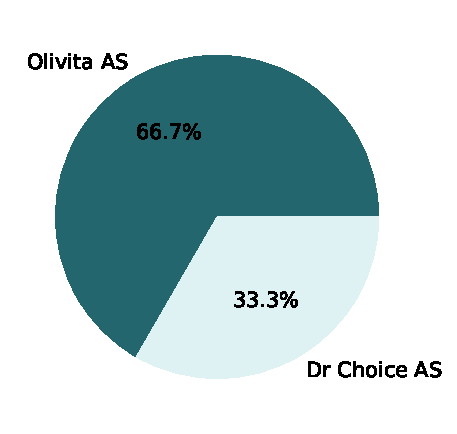
\includegraphics{18_SOK2030_mappeoppgave_2_V24_files/figure-pdf/cell-27-output-1.pdf}

\clearpage

\section {Appendix Python kode Oppgave 1 b}

\begin{Shaded}
\begin{Highlighting}[]
\NormalTok{a, b, Q\_O, Q\_C, c, f, p, Q }\OperatorTok{=}\NormalTok{ sp.symbols(}\StringTok{\textquotesingle{}a b Q\_O Q\_C c f p Q\textquotesingle{}}\NormalTok{)}

\NormalTok{demand }\OperatorTok{=}\NormalTok{ sp.Eq(p, a}\OperatorTok{{-}}\NormalTok{b}\OperatorTok{*}\NormalTok{(Q\_O}\OperatorTok{+}\NormalTok{Q\_C))}

\NormalTok{income }\OperatorTok{=}\NormalTok{ sp.Eq(p}\OperatorTok{*}\NormalTok{Q, Q}\OperatorTok{*}\NormalTok{(a}\OperatorTok{{-}}\NormalTok{b}\OperatorTok{*}\NormalTok{Q))}
\NormalTok{costs }\OperatorTok{=}\NormalTok{ Q}\OperatorTok{*}\NormalTok{c}\OperatorTok{{-}}\NormalTok{f}

\NormalTok{MR }\OperatorTok{=}\NormalTok{ sp.solve(sp.diff(income.rhs}\OperatorTok{{-}}\NormalTok{costs, Q), c)[}\DecValTok{0}\NormalTok{]}

\NormalTok{MR1 }\OperatorTok{=}\NormalTok{ sp.Eq(sp.diff((a}\OperatorTok{{-}}\NormalTok{b}\OperatorTok{*}\NormalTok{(Q\_O}\OperatorTok{+}\NormalTok{Q\_C))}\OperatorTok{*}\NormalTok{Q\_O}\OperatorTok{{-}}\NormalTok{f, Q\_O), c)}
\NormalTok{RF1  }\OperatorTok{=}\NormalTok{ sp.solve(MR1, Q\_O)[}\DecValTok{0}\NormalTok{]}

\NormalTok{MR2 }\OperatorTok{=}\NormalTok{ sp.Eq(sp.diff((a}\OperatorTok{{-}}\NormalTok{b}\OperatorTok{*}\NormalTok{(Q\_C}\OperatorTok{+}\NormalTok{Q\_O))}\OperatorTok{*}\NormalTok{Q\_C}\OperatorTok{{-}}\NormalTok{f, Q\_C), c)}
\NormalTok{RF2 }\OperatorTok{=}\NormalTok{ sp.solve(MR2, Q\_C)[}\DecValTok{0}\NormalTok{]}


\NormalTok{optimalt\_kvantum1 }\OperatorTok{=}\NormalTok{ sp.solve(sp.Eq(RF1.subs(Q\_C, RF2), Q\_O))[}\DecValTok{0}\NormalTok{][Q\_O]}

\NormalTok{optimalt\_kvantum2 }\OperatorTok{=}\NormalTok{ sp.solve(sp.Eq(RF2.subs(Q\_O, RF1), Q\_C))[}\DecValTok{0}\NormalTok{][Q\_C]}

\NormalTok{profitt\_1 }\OperatorTok{=}\NormalTok{ (demand.rhs}\OperatorTok{{-}}\NormalTok{costs).subs(Q, optimalt\_kvantum1)}


\NormalTok{markedspris }\OperatorTok{=} \BuiltInTok{round}\NormalTok{(}\BuiltInTok{float}\NormalTok{(sp.solve(demand.subs(\{a:}\DecValTok{990}\NormalTok{, b:}\DecValTok{1}\OperatorTok{/}\DecValTok{60}\NormalTok{, Q\_O:optimalt\_kvantum1, Q\_C:optimalt\_kvantum2, c: }\DecValTok{50}\NormalTok{\}), p)[}\DecValTok{0}\NormalTok{]),}\DecValTok{3}\NormalTok{)}

\NormalTok{profitt\_1 }\OperatorTok{=}\NormalTok{ (demand.rhs}\OperatorTok{{-}}\NormalTok{costs).subs(\{Q\_O: optimalt\_kvantum1, Q\_C: optimalt\_kvantum2, Q: optimalt\_kvantum1, f: }\DecValTok{3000000}\NormalTok{, a: }\DecValTok{990}\NormalTok{, b: }\DecValTok{1}\OperatorTok{/}\DecValTok{60}\NormalTok{, c: }\DecValTok{50}\NormalTok{\}) }
\NormalTok{profitt\_2 }\OperatorTok{=}\NormalTok{ (demand.rhs}\OperatorTok{{-}}\NormalTok{costs).subs(\{Q\_O: optimalt\_kvantum1, Q\_C: optimalt\_kvantum2, Q: optimalt\_kvantum2, f: }\DecValTok{3000000}\NormalTok{, a: }\DecValTok{990}\NormalTok{, b: }\DecValTok{1}\OperatorTok{/}\DecValTok{60}\NormalTok{, c: }\DecValTok{50}\NormalTok{\})}



\NormalTok{kvantum\_QO }\OperatorTok{=} \BuiltInTok{int}\NormalTok{(optimalt\_kvantum1.subs(\{a:}\DecValTok{990}\NormalTok{, b:}\DecValTok{1}\OperatorTok{/}\DecValTok{60}\NormalTok{, c:}\DecValTok{50}\NormalTok{, f:}\DecValTok{3000000}\NormalTok{\}))}
\NormalTok{kvantum\_QC }\OperatorTok{=} \BuiltInTok{int}\NormalTok{(optimalt\_kvantum2.subs(\{a:}\DecValTok{990}\NormalTok{, b:}\DecValTok{1}\OperatorTok{/}\DecValTok{60}\NormalTok{, c:}\DecValTok{50}\NormalTok{, f:}\DecValTok{3000000}\NormalTok{\}))}

\BuiltInTok{print}\NormalTok{(}\SpecialStringTok{f\textquotesingle{}\textquotesingle{}\textquotesingle{}Kvantum for Olivitas: }\SpecialCharTok{\{}\BuiltInTok{round}\NormalTok{(kvantum\_QO)}\SpecialCharTok{\}}\SpecialStringTok{ og kvantum for Dr Choice AS blir }\SpecialCharTok{\{}\BuiltInTok{round}\NormalTok{(kvantum\_QC)}\SpecialCharTok{\}}\SpecialStringTok{. }\CharTok{\textbackslash{}n}\SpecialStringTok{Det totale kvantumet i markedet er }\SpecialCharTok{\{}\BuiltInTok{round}\NormalTok{(kvantum\_olivitas}\OperatorTok{+}\NormalTok{kvantum\_choice)}\SpecialCharTok{\}}\SpecialStringTok{ til en Markedsprisen på }\SpecialCharTok{\{}\BuiltInTok{round}\NormalTok{(markedspris)}\SpecialCharTok{\}}\SpecialStringTok{.}\CharTok{\textbackslash{}n\textbackslash{}n}\SpecialStringTok{Profitten for selskapene er }\SpecialCharTok{\{}\BuiltInTok{round}\NormalTok{(profitt\_1)}\SpecialCharTok{\}}\SpecialStringTok{ for Olivitas og }\SpecialCharTok{\{}\BuiltInTok{round}\NormalTok{(profitt\_2)}\SpecialCharTok{\}}\SpecialStringTok{ for Dr Choice AS.\textquotesingle{}\textquotesingle{}\textquotesingle{}}\NormalTok{)}
\end{Highlighting}
\end{Shaded}

\begin{verbatim}
Kvantum for Olivitas: 18800 og kvantum for Dr Choice AS blir 18800. 
Det totale kvantumet i markedet er 42300 til en Markedsprisen på 363.

Profitten for selskapene er 2060363 for Olivitas og 2060363 for Dr Choice AS.
\end{verbatim}

\begin{Shaded}
\begin{Highlighting}[]
\NormalTok{display(RF1.subs(\{a:}\DecValTok{990}\NormalTok{, b:}\DecValTok{1}\OperatorTok{/}\DecValTok{60}\NormalTok{, c:}\DecValTok{50}\NormalTok{\}))}
\NormalTok{display(RF2.subs(\{a:}\DecValTok{990}\NormalTok{, b:}\DecValTok{1}\OperatorTok{/}\DecValTok{60}\NormalTok{, c:}\DecValTok{50}\NormalTok{\}))}
\end{Highlighting}
\end{Shaded}

$\displaystyle 28200.0 - 0.5 Q_{C}$

$\displaystyle 28200.0 - 0.5 Q_{O}$

\clearpage

\section {Appendix Python kode Oppgave 2 a}

\begin{Shaded}
\begin{Highlighting}[]
\NormalTok{a, b, q\_G, q\_B, q\_M, q\_BM, c, f, f\_G, f\_B, f\_M, f\_BM, p, Q, c\_G, c\_B, c\_M, c\_BM, pi\_G, pi\_B, pi\_M, pi\_BM }\OperatorTok{=}\NormalTok{ sp.symbols(}\StringTok{\textquotesingle{}a b q\_G q\_B q\_M q\_}\SpecialCharTok{\{BM\}}\StringTok{ c f f\_G f\_B f\_M f\_}\SpecialCharTok{\{BM\}}\StringTok{ p Q c\_G c\_B c\_M c\_}\SpecialCharTok{\{BM\}}\StringTok{ }\CharTok{\textbackslash{}u03C0}\StringTok{\_G }\CharTok{\textbackslash{}u03C0}\StringTok{\_B }\CharTok{\textbackslash{}u03C0}\StringTok{\_M }\CharTok{\textbackslash{}u03C0}\StringTok{\_BM\textquotesingle{}}\NormalTok{)}



\NormalTok{demand }\OperatorTok{=}\NormalTok{ sp.Eq(p, a}\OperatorTok{{-}}\NormalTok{b}\OperatorTok{*}\NormalTok{(Q))}

\NormalTok{income }\OperatorTok{=}\NormalTok{ sp.Eq(p}\OperatorTok{*}\NormalTok{Q, Q}\OperatorTok{*}\NormalTok{(a}\OperatorTok{{-}}\NormalTok{b}\OperatorTok{*}\NormalTok{Q))}
\NormalTok{costs }\OperatorTok{=}\NormalTok{ Q}\OperatorTok{*}\NormalTok{c}\OperatorTok{+}\NormalTok{f}




\NormalTok{profitt\_G }\OperatorTok{=}\NormalTok{ sp.Eq(pi\_G, demand.rhs.subs(Q, q\_G}\OperatorTok{+}\NormalTok{q\_B}\OperatorTok{+}\NormalTok{q\_M)}\OperatorTok{*}\NormalTok{q\_G}\OperatorTok{{-}}\NormalTok{costs.subs(\{Q:q\_G, c:c\_G, f:f\_G\}))}
\NormalTok{profitt\_B }\OperatorTok{=}\NormalTok{ sp.Eq(pi\_B, demand.rhs.subs(Q, q\_G}\OperatorTok{+}\NormalTok{q\_B}\OperatorTok{+}\NormalTok{q\_M)}\OperatorTok{*}\NormalTok{q\_B}\OperatorTok{{-}}\NormalTok{costs.subs(\{Q:q\_B, c:c\_B, f:f\_B\}))}
\NormalTok{profitt\_M }\OperatorTok{=}\NormalTok{ sp.Eq(pi\_M, demand.rhs.subs(Q, q\_G}\OperatorTok{+}\NormalTok{q\_B}\OperatorTok{+}\NormalTok{q\_M)}\OperatorTok{*}\NormalTok{q\_M}\OperatorTok{{-}}\NormalTok{costs.subs(\{Q:q\_M, c:c\_M, f:f\_M\}))}
\end{Highlighting}
\end{Shaded}

\begin{Shaded}
\begin{Highlighting}[]
\NormalTok{derivert\_profitt\_G }\OperatorTok{=}\NormalTok{ sp.diff(profitt\_G.rhs, q\_G)}
\NormalTok{derivert\_profitt\_B }\OperatorTok{=}\NormalTok{ sp.diff(profitt\_B.rhs, q\_B)}
\NormalTok{derivert\_profitt\_M }\OperatorTok{=}\NormalTok{ sp.diff(profitt\_M.rhs, q\_M)}

\NormalTok{solved }\OperatorTok{=}\NormalTok{ sp.solve([derivert\_profitt\_G, derivert\_profitt\_B, derivert\_profitt\_M], [q\_G, q\_B, q\_M])}
\end{Highlighting}
\end{Shaded}

\begin{Shaded}
\begin{Highlighting}[]
\NormalTok{a\_num }\OperatorTok{=} \DecValTok{175}
\NormalTok{b\_num }\OperatorTok{=} \DecValTok{4}
\NormalTok{c\_M\_num }\OperatorTok{=} \DecValTok{7}
\NormalTok{c\_B\_num }\OperatorTok{=} \DecValTok{10}
\NormalTok{c\_G\_num }\OperatorTok{=} \DecValTok{10}
\NormalTok{f\_G\_num }\OperatorTok{=} \DecValTok{300}
\NormalTok{f\_B\_num }\OperatorTok{=} \DecValTok{300}
\NormalTok{f\_M\_num }\OperatorTok{=} \DecValTok{300}
\NormalTok{f\_BM\_num }\OperatorTok{=} \DecValTok{500}
\NormalTok{c\_BM\_num }\OperatorTok{=} \DecValTok{7}

\NormalTok{cournot }\OperatorTok{=}\NormalTok{ sp.lambdify(}
\NormalTok{    (a, b, c\_G, c\_B, c\_M), }
\NormalTok{    (solved[q\_G], solved[q\_B], solved[q\_M]))}
\NormalTok{kvantum\_G\_before\_cournot, kvantum\_B\_before\_cournot, kvantum\_M\_before\_cournot }\OperatorTok{=}\NormalTok{ cournot(a\_num, b\_num, c\_G\_num, c\_B\_num, c\_M\_num)}

\NormalTok{markedspris\_before\_cournot }\OperatorTok{=}\NormalTok{ demand.rhs.subs(\{a:a\_num, b:b\_num, Q:kvantum\_G\_before\_cournot}\OperatorTok{+}\NormalTok{kvantum\_B\_before\_cournot}\OperatorTok{+}\NormalTok{kvantum\_M\_before\_cournot\})}

\NormalTok{profitt\_G\_num }\OperatorTok{=} \BuiltInTok{round}\NormalTok{(}\BuiltInTok{float}\NormalTok{(profitt\_G.rhs.subs(\{q\_G:kvantum\_G\_before\_cournot, q\_B:kvantum\_B\_before\_cournot, q\_M:kvantum\_M\_before\_cournot, c\_G:c\_G\_num, a:a\_num, b:b\_num, p:markedspris\_before\_cournot, f\_G:f\_G\_num\})),}\DecValTok{2}\NormalTok{)}
\NormalTok{profitt\_B\_num }\OperatorTok{=} \BuiltInTok{round}\NormalTok{(}\BuiltInTok{float}\NormalTok{(profitt\_B.rhs.subs(\{q\_G:kvantum\_G\_before\_cournot, q\_B:kvantum\_B\_before\_cournot, q\_M:kvantum\_M\_before\_cournot, c\_B:c\_B\_num, a:a\_num, b:b\_num, p:markedspris\_before\_cournot, f\_B:f\_B\_num\})),}\DecValTok{2}\NormalTok{)}
\NormalTok{profitt\_M\_num }\OperatorTok{=} \BuiltInTok{round}\NormalTok{(}\BuiltInTok{float}\NormalTok{(profitt\_M.rhs.subs(\{q\_G:kvantum\_G\_before\_cournot, q\_B:kvantum\_B\_before\_cournot, q\_M:kvantum\_M\_before\_cournot, c\_M:c\_M\_num, a:a\_num, b:b\_num, p:markedspris\_before\_cournot, f\_M:f\_M\_num\})),}\DecValTok{2}\NormalTok{)}
\end{Highlighting}
\end{Shaded}

\begin{Shaded}
\begin{Highlighting}[]
\NormalTok{fig, ax }\OperatorTok{=}\NormalTok{ plt.subplots()}

\NormalTok{labels }\OperatorTok{=}\NormalTok{ [}\StringTok{\textquotesingle{}Graff Brygghus\textquotesingle{}}\NormalTok{, }\StringTok{\textquotesingle{}Bryggeri 13\textquotesingle{}}\NormalTok{, }\StringTok{\textquotesingle{}Mack Mikrobryggeri\textquotesingle{}}\NormalTok{]}
\NormalTok{sizes }\OperatorTok{=}\NormalTok{ [kvantum\_G\_before\_cournot, kvantum\_B\_before\_cournot, kvantum\_M\_before\_cournot]}

\NormalTok{ax.pie(sizes, labels}\OperatorTok{=}\NormalTok{labels, autopct}\OperatorTok{=}\StringTok{\textquotesingle{}}\SpecialCharTok{\%1.1f\%\%}\StringTok{\textquotesingle{}}\NormalTok{, colors}\OperatorTok{=}\NormalTok{[}\StringTok{\textquotesingle{}\#def2f4\textquotesingle{}}\NormalTok{, }\StringTok{\textquotesingle{}\#3599a4\textquotesingle{}}\NormalTok{, }\StringTok{\textquotesingle{}\#24666d\textquotesingle{}}\NormalTok{])}
\CommentTok{\#plt.savefig(\textquotesingle{}dokumentobjekter/figurer/markedsandel\_mikrobryggerier.png\textquotesingle{}, dpi=300, bbox\_inches=\textquotesingle{}tight\textquotesingle{})}
\NormalTok{plt.show()}\OperatorTok{;}
\end{Highlighting}
\end{Shaded}

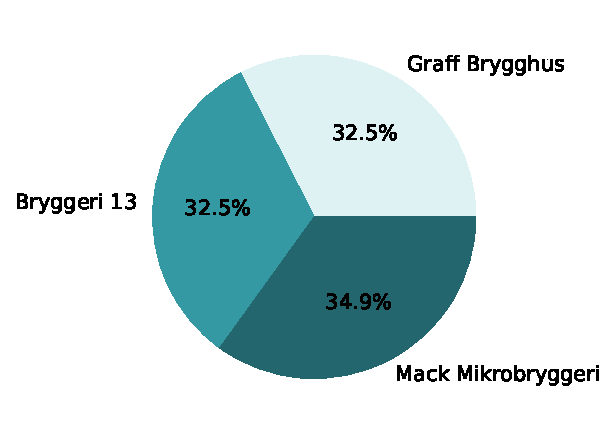
\includegraphics{18_SOK2030_mappeoppgave_2_V24_files/figure-pdf/cell-33-output-1.pdf}

\begin{Shaded}
\begin{Highlighting}[]
\NormalTok{profitt\_G\_before\_cournot }\OperatorTok{=}\NormalTok{ profitt\_G.subs(\{q\_G:kvantum\_G\_before\_cournot, q\_B:kvantum\_B\_before\_cournot, q\_M:kvantum\_M\_before\_cournot, c\_G:c\_G\_num, a:a\_num, b:b\_num, p:markedspris\_before\_cournot, f\_G:f\_G\_num\})}


\NormalTok{profitt\_B\_before\_cournot }\OperatorTok{=}\NormalTok{ profitt\_B.subs(\{q\_G:kvantum\_G\_before\_cournot, q\_B:kvantum\_B\_before\_cournot, q\_M:kvantum\_M\_before\_cournot, c\_B:c\_B\_num, a:a\_num, b:b\_num, p:markedspris\_before\_cournot, f\_B:f\_B\_num\})}


\NormalTok{profitt\_M\_before\_cournot }\OperatorTok{=}\NormalTok{ profitt\_M.subs(\{q\_G:kvantum\_G\_before\_cournot, q\_B:kvantum\_B\_before\_cournot, q\_M:kvantum\_M\_before\_cournot, c\_M:c\_M\_num, a:a\_num, b:b\_num, p:markedspris\_before\_cournot, f\_M:f\_M\_num\})}
\end{Highlighting}
\end{Shaded}

\begin{Shaded}
\begin{Highlighting}[]
\NormalTok{profitt\_G\_etter\_cournot }\OperatorTok{=}\NormalTok{ sp.Eq(pi\_G, demand.rhs.subs(Q, q\_G}\OperatorTok{+}\NormalTok{q\_BM)}\OperatorTok{*}\NormalTok{q\_G}\OperatorTok{{-}}\NormalTok{costs.subs(\{Q:q\_G, c:c\_G, f:f\_G\}))}
\NormalTok{profitt\_MB\_etter\_cournot }\OperatorTok{=}\NormalTok{ sp.Eq(pi\_BM, demand.rhs.subs(Q, q\_G}\OperatorTok{+}\NormalTok{q\_BM)}\OperatorTok{*}\NormalTok{q\_BM}\OperatorTok{{-}}\NormalTok{costs.subs(\{Q:q\_BM, c:c\_BM, f:f\_BM\}))}
\end{Highlighting}
\end{Shaded}

\begin{Shaded}
\begin{Highlighting}[]
\NormalTok{derivert\_profitt\_G\_etter\_cournot }\OperatorTok{=}\NormalTok{ sp.diff(profitt\_G\_etter\_cournot.rhs, q\_G)}
\NormalTok{derivert\_profitt\_MB\_etter\_cournot }\OperatorTok{=}\NormalTok{ sp.diff(profitt\_MB\_etter\_cournot.rhs, q\_BM)}

\NormalTok{solved\_etter\_cournot }\OperatorTok{=}\NormalTok{ sp.solve([derivert\_profitt\_G\_etter\_cournot, derivert\_profitt\_MB\_etter\_cournot], [q\_G, q\_BM])}
\end{Highlighting}
\end{Shaded}

\begin{Shaded}
\begin{Highlighting}[]
\NormalTok{cournot\_etter\_cournot }\OperatorTok{=}\NormalTok{ sp.lambdify(}
\NormalTok{    (a, b, c\_G, c\_BM), }
\NormalTok{    (solved\_etter\_cournot[q\_G], solved\_etter\_cournot[q\_BM]))}
    
\NormalTok{kvantum\_G\_etter\_cournot, kvantum\_BM\_etter\_cournot }\OperatorTok{=}\NormalTok{ cournot\_etter\_cournot(a\_num, b\_num, c\_G\_num, c\_BM\_num)}
\NormalTok{markedspris\_etter\_cournot }\OperatorTok{=}\NormalTok{ demand.rhs.subs(\{a:a\_num, b:b\_num, Q:kvantum\_G\_etter\_cournot}\OperatorTok{+}\NormalTok{kvantum\_BM\_etter\_cournot\})}

\NormalTok{profitt\_G\_etter\_cournot }\OperatorTok{=} \BuiltInTok{round}\NormalTok{(}\BuiltInTok{float}\NormalTok{(profitt\_G\_etter\_cournot.rhs.subs(\{q\_G:kvantum\_G\_etter\_cournot, q\_BM:kvantum\_BM\_etter\_cournot, c\_G:c\_G\_num, a:a\_num, b:b\_num, f\_G:f\_G\_num\})),}\DecValTok{2}\NormalTok{)}
\NormalTok{profitt\_BM\_etter\_cournot }\OperatorTok{=} \BuiltInTok{round}\NormalTok{(}\BuiltInTok{float}\NormalTok{(profitt\_MB\_etter\_cournot.rhs.subs(\{q\_G:kvantum\_G\_etter\_cournot, q\_BM:kvantum\_BM\_etter\_cournot, c\_BM:c\_BM\_num, a:a\_num, b:b\_num, f\_BM:f\_BM\_num\})),}\DecValTok{2}\NormalTok{)}
\end{Highlighting}
\end{Shaded}

\begin{Shaded}
\begin{Highlighting}[]
\NormalTok{fig, ax }\OperatorTok{=}\NormalTok{ plt.subplots()}

\NormalTok{labels }\OperatorTok{=}\NormalTok{ [}\StringTok{\textquotesingle{}Graff Brygghus\textquotesingle{}}\NormalTok{, }\StringTok{\textquotesingle{}Mack Mikrobryggeri\textquotesingle{}}\NormalTok{]}
\NormalTok{sizes }\OperatorTok{=}\NormalTok{ [kvantum\_G\_etter\_cournot, kvantum\_BM\_etter\_cournot]}

\NormalTok{ax.pie(sizes, labels}\OperatorTok{=}\NormalTok{labels, autopct}\OperatorTok{=}\StringTok{\textquotesingle{}}\SpecialCharTok{\%1.1f\%\%}\StringTok{\textquotesingle{}}\NormalTok{, colors}\OperatorTok{=}\NormalTok{[}\StringTok{\textquotesingle{}\#def2f4\textquotesingle{}}\NormalTok{, }\StringTok{\textquotesingle{}\#24666d\textquotesingle{}}\NormalTok{])}
\CommentTok{\#plt.savefig(\textquotesingle{}dokumentobjekter/figurer/markedsandel\_mikrobryggerier\_fusjon.png\textquotesingle{}, dpi=300, bbox\_inches=\textquotesingle{}tight\textquotesingle{})}
\NormalTok{plt.show()}\OperatorTok{;}
\end{Highlighting}
\end{Shaded}

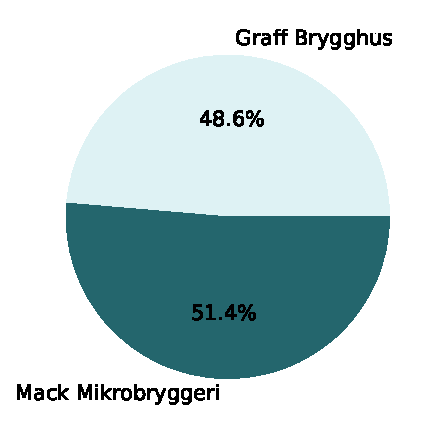
\includegraphics{18_SOK2030_mappeoppgave_2_V24_files/figure-pdf/cell-38-output-1.pdf}

\begin{Shaded}
\begin{Highlighting}[]
\NormalTok{q\_BM, q\_G, p, c, f, pi\_G, pi\_BM}\OperatorTok{=}\NormalTok{ sp.symbols(}\StringTok{\textquotesingle{}q\_BM q\_G p c f }\CharTok{\textbackslash{}u03C0}\StringTok{\_G }\CharTok{\textbackslash{}u03C0}\StringTok{\_BM\textquotesingle{}}\NormalTok{)}

\NormalTok{Invers\_etterspors }\OperatorTok{=}\NormalTok{ sp.Eq(p, (}\DecValTok{175}\OperatorTok{{-}}\NormalTok{(}\DecValTok{4}\NormalTok{)}\OperatorTok{*}\NormalTok{(q\_G}\OperatorTok{+}\NormalTok{q\_BM)))}


\NormalTok{profitt\_1\_eq\_stack }\OperatorTok{=}\NormalTok{ sp.Eq(pi\_BM, (Invers\_etterspors.rhs}\OperatorTok{{-}}\DecValTok{7}\NormalTok{)}\OperatorTok{*}\NormalTok{q\_G}\OperatorTok{{-}}\DecValTok{500}\NormalTok{)}
\NormalTok{profitt\_2\_eq\_stack }\OperatorTok{=}\NormalTok{ sp.Eq(pi\_G, (Invers\_etterspors.rhs}\OperatorTok{{-}}\DecValTok{10}\NormalTok{)}\OperatorTok{*}\NormalTok{q\_BM}\OperatorTok{{-}}\DecValTok{300}\NormalTok{)}


\NormalTok{derivert\_profitt\_2\_stack }\OperatorTok{=}\NormalTok{ sp.diff(profitt\_2\_eq\_stack.rhs, q\_BM)}

\NormalTok{reaksjon\_BM\_stack }\OperatorTok{=}\NormalTok{ sp.solve(derivert\_profitt\_2\_stack, q\_BM)[}\DecValTok{0}\NormalTok{]}

\NormalTok{profitt\_1\_eq\_stack }\OperatorTok{=}\NormalTok{ profitt\_1\_eq\_stack.subs(q\_BM, reaksjon\_BM\_stack)}

\NormalTok{derivert\_profitt1\_stack }\OperatorTok{=}\NormalTok{ sp.diff(profitt\_1\_eq\_stack.rhs, q\_G) }\CommentTok{\#kvantum for kvantum og bryggeri}

\NormalTok{kvantum\_BM\_stack }\OperatorTok{=}\NormalTok{ sp.solve(derivert\_profitt1\_stack, q\_G)[}\DecValTok{0}\NormalTok{]}

\CommentTok{\#setter inn kvantum i reaksjonsfunksjonen til Dr Choice AS}
\NormalTok{kvantum\_G\_stack }\OperatorTok{=}\NormalTok{ reaksjon\_BM\_stack.subs(q\_G, kvantum\_BM\_stack)}\CommentTok{\#Kvantum for mack og bryggeri 13}
\NormalTok{markedspris\_stack }\OperatorTok{=}\NormalTok{ Invers\_etterspors.rhs.subs(\{q\_G:kvantum\_BM\_stack, q\_BM:kvantum\_G\_stack\})}
\NormalTok{profitt\_BM\_stack }\OperatorTok{=} \BuiltInTok{float}\NormalTok{(profitt\_1\_eq\_stack.rhs.subs(q\_G, kvantum\_BM\_stack).subs(q\_BM, kvantum\_G\_stack))}

\NormalTok{profitt\_G\_stack }\OperatorTok{=} \BuiltInTok{float}\NormalTok{(profitt\_2\_eq\_stack.rhs.subs(q\_BM, kvantum\_G\_stack).subs(q\_G, kvantum\_BM\_stack))}

\BuiltInTok{print}\NormalTok{(}\SpecialStringTok{f\textquotesingle{}\textquotesingle{}\textquotesingle{}Kvantum for fusjonert Mack: }\SpecialCharTok{\{}\BuiltInTok{round}\NormalTok{(kvantum\_BM\_stack,}\DecValTok{2}\NormalTok{)}\SpecialCharTok{\}}\SpecialStringTok{ og Kvantum for Graff Brygghus: }\SpecialCharTok{\{}\BuiltInTok{round}\NormalTok{(kvantum\_G\_stack, }\DecValTok{2}\NormalTok{)}\SpecialCharTok{\}}\SpecialStringTok{. }\CharTok{\textbackslash{}n}\SpecialStringTok{Det totale kvantumet i markedet er }\SpecialCharTok{\{}\BuiltInTok{round}\NormalTok{(kvantum\_BM\_stack}\OperatorTok{+}\NormalTok{kvantum\_G\_stack, }\DecValTok{2}\NormalTok{)}\SpecialCharTok{\}}\SpecialStringTok{ til en Markedsprisen på }\SpecialCharTok{\{}\BuiltInTok{round}\NormalTok{(markedspris\_stack, }\DecValTok{2}\NormalTok{)}\SpecialCharTok{\}}\SpecialStringTok{.}\CharTok{\textbackslash{}n\textbackslash{}n}\SpecialStringTok{Profitten for selskapene er }\SpecialCharTok{\{}\BuiltInTok{round}\NormalTok{(profitt\_BM\_stack, }\DecValTok{2}\NormalTok{)}\SpecialCharTok{\}}\SpecialStringTok{ for fusjonert Mack og }\SpecialCharTok{\{}\BuiltInTok{round}\NormalTok{(profitt\_G\_stack, }\DecValTok{2}\NormalTok{)}\SpecialCharTok{\}}\SpecialStringTok{ for Graff Brygghus.\textquotesingle{}\textquotesingle{}\textquotesingle{}}\NormalTok{)}
\end{Highlighting}
\end{Shaded}

\begin{verbatim}
Kvantum for fusjonert Mack: 21.38 og Kvantum for Graff Brygghus: 9.94. 
Det totale kvantumet i markedet er 31.31 til en Markedsprisen på 49.75.

Profitten for selskapene er 413.78 for fusjonert Mack og 95.02 for Graff Brygghus.
\end{verbatim}

\begin{Shaded}
\begin{Highlighting}[]
\NormalTok{fig, ax }\OperatorTok{=}\NormalTok{ plt.subplots()}

\NormalTok{labels }\OperatorTok{=}\NormalTok{ [}\StringTok{\textquotesingle{}Graff Brygghus\textquotesingle{}}\NormalTok{, }\StringTok{\textquotesingle{}Mack Mikrobryggeri\textquotesingle{}}\NormalTok{]}
\NormalTok{sizes }\OperatorTok{=}\NormalTok{ [kvantum\_G\_stack, kvantum\_BM\_stack]}

\NormalTok{ax.pie(sizes, labels}\OperatorTok{=}\NormalTok{labels, autopct}\OperatorTok{=}\StringTok{\textquotesingle{}}\SpecialCharTok{\%1.1f\%\%}\StringTok{\textquotesingle{}}\NormalTok{, colors}\OperatorTok{=}\NormalTok{[}\StringTok{\textquotesingle{}\#def2f4\textquotesingle{}}\NormalTok{, }\StringTok{\textquotesingle{}\#24666d\textquotesingle{}}\NormalTok{])}
\CommentTok{\#plt.savefig(\textquotesingle{}dokumentobjekter/figurer/markedsandel\_mikrobryggerier\_fusjon\_stackel.png\textquotesingle{}, dpi=300, bbox\_inches=\textquotesingle{}tight\textquotesingle{})}
\NormalTok{plt.show()}\OperatorTok{;}
\end{Highlighting}
\end{Shaded}

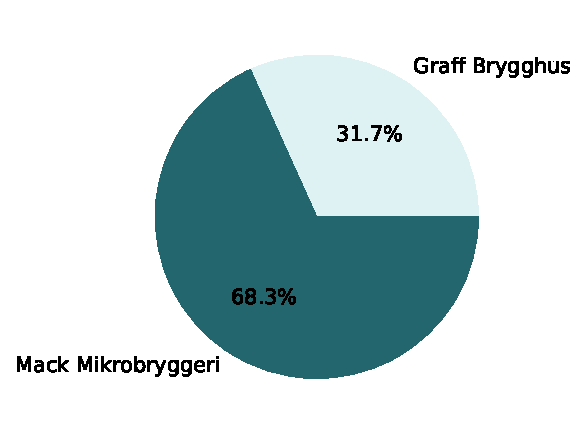
\includegraphics{18_SOK2030_mappeoppgave_2_V24_files/figure-pdf/cell-40-output-1.pdf}

\begin{Shaded}
\begin{Highlighting}[]
\NormalTok{tbl1 }\OperatorTok{=} \VerbatimStringTok{rf"""}
\VerbatimStringTok{\textbackslash{}begin}\CharTok{\{\{}\VerbatimStringTok{table}\CharTok{\}\}}\VerbatimStringTok{[h]}
\VerbatimStringTok{\textbackslash{}centering}
\VerbatimStringTok{\textbackslash{}begin}\CharTok{\{\{}\VerbatimStringTok{tabular}\CharTok{\}\}\{\{}\VerbatimStringTok{|l|l|l|l|}\CharTok{\}\}}
\VerbatimStringTok{\textbackslash{}hline}
\VerbatimStringTok{\textbackslash{}rowcolor}\CharTok{\{\{}\VerbatimStringTok{cornflowerblue}\CharTok{\}\}}\VerbatimStringTok{ \textbackslash{}textbf}\CharTok{\{\{}\VerbatimStringTok{Bedrift}\CharTok{\}\}}\VerbatimStringTok{ \& \textbackslash{}textbf}\CharTok{\{\{}\VerbatimStringTok{Variabel}\CharTok{\}\}}\VerbatimStringTok{ \& \textbackslash{}textbf}\CharTok{\{\{}\VerbatimStringTok{Cournot}\CharTok{\}\}}\VerbatimStringTok{ \& \textbackslash{}textbf}\CharTok{\{\{}\VerbatimStringTok{Stackelberg}\CharTok{\}\}}\VerbatimStringTok{ \textbackslash{}\textbackslash{} \textbackslash{}hline}
\VerbatimStringTok{\textbackslash{}rowcolor}\CharTok{\{\{}\VerbatimStringTok{lighterblue}\CharTok{\}\}}\VerbatimStringTok{ Mack Mikrobryggeri      \& Profitt                  \& $}\SpecialCharTok{\{}\NormalTok{profitt\_M\_num}\OperatorTok{*}\DecValTok{1000}\SpecialCharTok{\}}\VerbatimStringTok{\textasciitilde{}kr$             \& {-}           \textbackslash{}\textbackslash{} \textbackslash{}hline}
\VerbatimStringTok{\textbackslash{}rowcolor}\CharTok{\{\{}\VerbatimStringTok{lighterblue}\CharTok{\}\}}\VerbatimStringTok{ Bryggeri 13  \& Profitt                  \& $}\SpecialCharTok{\{}\NormalTok{profitt\_B\_num}\OperatorTok{*}\DecValTok{1000}\SpecialCharTok{\}}\VerbatimStringTok{\textasciitilde{}kr$             \& {-}           \textbackslash{}\textbackslash{} \textbackslash{}hline}
\VerbatimStringTok{\textbackslash{}rowcolor}\CharTok{\{\{}\VerbatimStringTok{lighterblue}\CharTok{\}\}}\VerbatimStringTok{ Graff Brygghus  \& Profitt                  \& $}\SpecialCharTok{\{}\NormalTok{profitt\_G\_num}\OperatorTok{*}\DecValTok{1000}\SpecialCharTok{\}}\VerbatimStringTok{\textasciitilde{}kr$             \& {-}           \textbackslash{}\textbackslash{} \textbackslash{}hline }
\VerbatimStringTok{\textbackslash{}textbf}\CharTok{\{\{}\VerbatimStringTok{Total}\CharTok{\}\}}\VerbatimStringTok{  \& {-}                  \& $}\SpecialCharTok{\{}\NormalTok{(profitt\_G\_num}\OperatorTok{*}\DecValTok{1000}\NormalTok{) }\OperatorTok{+}\NormalTok{ (profitt\_B\_num}\OperatorTok{*}\DecValTok{1000}\NormalTok{) }\OperatorTok{+}\NormalTok{ (profitt\_M\_num}\OperatorTok{*}\DecValTok{1000}\NormalTok{)}\SpecialCharTok{\}}\VerbatimStringTok{\textasciitilde{}kr$             \& {-}           \textbackslash{}\textbackslash{} \textbackslash{}hline}
\VerbatimStringTok{\textbackslash{}rowcolor}\CharTok{\{\{}\VerbatimStringTok{lightblue}\CharTok{\}\}}\VerbatimStringTok{ Mack Mikrobryggeri      \& Kvantum                  \& $}\SpecialCharTok{\{}\NormalTok{kvantum\_M\_before\_cournot}\OperatorTok{*}\DecValTok{1000}\SpecialCharTok{\}}\VerbatimStringTok{$             \& {-}           \textbackslash{}\textbackslash{} \textbackslash{}hline}
\VerbatimStringTok{\textbackslash{}rowcolor}\CharTok{\{\{}\VerbatimStringTok{lightblue}\CharTok{\}\}}\VerbatimStringTok{ Bryggeri 13  \& Kvantum                  \& $}\SpecialCharTok{\{}\NormalTok{kvantum\_B\_before\_cournot}\OperatorTok{*}\DecValTok{1000}\SpecialCharTok{\}}\VerbatimStringTok{$             \& {-}           \textbackslash{}\textbackslash{} \textbackslash{}hline}
\VerbatimStringTok{\textbackslash{}rowcolor}\CharTok{\{\{}\VerbatimStringTok{lightblue}\CharTok{\}\}}\VerbatimStringTok{ Graff Brygghus  \& Kvantum                  \& $}\SpecialCharTok{\{}\NormalTok{kvantum\_G\_before\_cournot}\OperatorTok{*}\DecValTok{1000}\SpecialCharTok{\}}\VerbatimStringTok{$             \& {-}           \textbackslash{}\textbackslash{} \textbackslash{}hline }
\VerbatimStringTok{\textbackslash{}textbf}\CharTok{\{\{}\VerbatimStringTok{Total}\CharTok{\}\}}\VerbatimStringTok{  \& {-}                  \& $}\SpecialCharTok{\{}\NormalTok{(kvantum\_M\_before\_cournot}\OperatorTok{*}\DecValTok{1000}\NormalTok{)}\OperatorTok{+}\NormalTok{(kvantum\_B\_before\_cournot}\OperatorTok{*}\DecValTok{1000}\NormalTok{)}\OperatorTok{+}\NormalTok{(kvantum\_G\_before\_cournot}\OperatorTok{*}\DecValTok{1000}\NormalTok{)}\SpecialCharTok{\}}\VerbatimStringTok{$             \& {-}          \textbackslash{}\textbackslash{} \textbackslash{}hline}
\VerbatimStringTok{{-} \& \textbackslash{}textbf}\CharTok{\{\{}\VerbatimStringTok{Markedspris}\CharTok{\}\}}\VerbatimStringTok{ \& $}\SpecialCharTok{\{}\BuiltInTok{round}\NormalTok{(markedspris\_before\_cournot,}\DecValTok{2}\NormalTok{)}\SpecialCharTok{\}}\VerbatimStringTok{\textasciitilde{}kr$ \& {-} \textbackslash{}\textbackslash{} \textbackslash{}hline}
\VerbatimStringTok{\textbackslash{}rowcolor}\CharTok{\{\{}\VerbatimStringTok{cornflowerblue}\CharTok{\}\}}\VerbatimStringTok{ \textbackslash{}textbf}\CharTok{\{\{}\VerbatimStringTok{Bedrift etter fusjon}\CharTok{\}\}}\VerbatimStringTok{ \& \textbackslash{}textbf}\CharTok{\{\{}\VerbatimStringTok{Variabel}\CharTok{\}\}}\VerbatimStringTok{ \& \textbackslash{}textbf}\CharTok{\{\{}\VerbatimStringTok{Cournot}\CharTok{\}\}}\VerbatimStringTok{ \& \textbackslash{}textbf}\CharTok{\{\{}\VerbatimStringTok{Stackelberg}\CharTok{\}\}}\VerbatimStringTok{ \textbackslash{}\textbackslash{} \textbackslash{}hline}
\VerbatimStringTok{\textbackslash{}rowcolor}\CharTok{\{\{}\VerbatimStringTok{lighterblue}\CharTok{\}\}}\VerbatimStringTok{ Fusjonert Mack og Bryggeri      \& Profitt                  \& $}\SpecialCharTok{\{}\NormalTok{profitt\_BM\_etter\_cournot}\OperatorTok{*}\DecValTok{1000}\SpecialCharTok{\}}\VerbatimStringTok{\textasciitilde{}kr$             \& $}\SpecialCharTok{\{}\BuiltInTok{round}\NormalTok{(profitt\_BM\_stack}\OperatorTok{*}\DecValTok{1000}\NormalTok{,}\DecValTok{2}\NormalTok{)}\SpecialCharTok{\}}\VerbatimStringTok{\textasciitilde{}kr$           \textbackslash{}\textbackslash{} \textbackslash{}hline}
\VerbatimStringTok{\textbackslash{}rowcolor}\CharTok{\{\{}\VerbatimStringTok{lighterblue}\CharTok{\}\}}\VerbatimStringTok{ Graff Brygghus  \& Profitt                  \& $}\SpecialCharTok{\{}\BuiltInTok{float}\NormalTok{(profitt\_G\_etter\_cournot)}\OperatorTok{*}\DecValTok{1000}\SpecialCharTok{\}}\VerbatimStringTok{\textasciitilde{}kr$             \& $}\SpecialCharTok{\{}\BuiltInTok{round}\NormalTok{(profitt\_G\_stack}\OperatorTok{*}\DecValTok{1000}\NormalTok{,}\DecValTok{2}\NormalTok{)}\SpecialCharTok{\}}\VerbatimStringTok{\textasciitilde{}kr$           \textbackslash{}\textbackslash{} \textbackslash{}hline }
\VerbatimStringTok{\textbackslash{}textbf}\CharTok{\{\{}\VerbatimStringTok{Total}\CharTok{\}\}}\VerbatimStringTok{  \& {-}                  \& $}\SpecialCharTok{\{}\NormalTok{(profitt\_BM\_etter\_cournot}\OperatorTok{*}\DecValTok{1000}\NormalTok{)}\OperatorTok{+}\NormalTok{(profitt\_G\_etter\_cournot}\OperatorTok{*}\DecValTok{1000}\NormalTok{)}\SpecialCharTok{\}}\VerbatimStringTok{\textasciitilde{}kr$             \& $}\SpecialCharTok{\{}\BuiltInTok{round}\NormalTok{((profitt\_G\_stack}\OperatorTok{*}\DecValTok{1000}\NormalTok{)}\OperatorTok{+}\NormalTok{(profitt\_BM\_stack)}\OperatorTok{*}\DecValTok{1000}\NormalTok{,}\DecValTok{2}\NormalTok{)}\SpecialCharTok{\}}\VerbatimStringTok{\textasciitilde{}kr$           \textbackslash{}\textbackslash{} \textbackslash{}hline}
\VerbatimStringTok{\textbackslash{}rowcolor}\CharTok{\{\{}\VerbatimStringTok{lightblue}\CharTok{\}\}}\VerbatimStringTok{ Fusjonert Mack og Bryggeri      \& Kvantum                  \& $}\SpecialCharTok{\{}\NormalTok{kvantum\_BM\_etter\_cournot}\OperatorTok{*}\DecValTok{1000}\SpecialCharTok{\}}\VerbatimStringTok{$             \& $}\SpecialCharTok{\{}\BuiltInTok{round}\NormalTok{(kvantum\_BM\_stack}\OperatorTok{*}\DecValTok{1000}\NormalTok{,}\DecValTok{2}\NormalTok{)}\SpecialCharTok{\}}\VerbatimStringTok{$           \textbackslash{}\textbackslash{} \textbackslash{}hline}
\VerbatimStringTok{\textbackslash{}rowcolor}\CharTok{\{\{}\VerbatimStringTok{lightblue}\CharTok{\}\}}\VerbatimStringTok{ Graff Brygghus  \& Kvantum                  \& $}\SpecialCharTok{\{}\NormalTok{kvantum\_G\_etter\_cournot}\OperatorTok{*}\DecValTok{1000}\SpecialCharTok{\}}\VerbatimStringTok{$             \& $}\SpecialCharTok{\{}\BuiltInTok{round}\NormalTok{((kvantum\_G\_stack}\OperatorTok{*}\DecValTok{1000}\NormalTok{),}\DecValTok{2}\NormalTok{)}\SpecialCharTok{\}}\VerbatimStringTok{$           \textbackslash{}\textbackslash{} \textbackslash{}hline}
\VerbatimStringTok{\textbackslash{}textbf}\CharTok{\{\{}\VerbatimStringTok{Total}\CharTok{\}\}}\VerbatimStringTok{  \& {-}                  \& $}\SpecialCharTok{\{}\NormalTok{kvantum\_BM\_etter\_cournot}\OperatorTok{*}\DecValTok{1000}\OperatorTok{+}\NormalTok{kvantum\_G\_etter\_cournot}\OperatorTok{*}\DecValTok{1000}\SpecialCharTok{\}}\VerbatimStringTok{$             \& $}\SpecialCharTok{\{}\BuiltInTok{round}\NormalTok{((kvantum\_BM\_stack}\OperatorTok{+}\NormalTok{kvantum\_G\_stack)}\OperatorTok{*}\DecValTok{1000}\NormalTok{,}\DecValTok{2}\NormalTok{)}\SpecialCharTok{\}}\VerbatimStringTok{$           \textbackslash{}\textbackslash{} \textbackslash{}hline}
\VerbatimStringTok{{-} \& \textbackslash{}textbf}\CharTok{\{\{}\VerbatimStringTok{Markedspris}\CharTok{\}\}}\VerbatimStringTok{ \& $}\SpecialCharTok{\{}\BuiltInTok{round}\NormalTok{(}\BuiltInTok{float}\NormalTok{(markedspris\_etter\_cournot),}\DecValTok{2}\NormalTok{)}\SpecialCharTok{\}}\VerbatimStringTok{\textasciitilde{}kr$ \& $}\SpecialCharTok{\{}\BuiltInTok{round}\NormalTok{(markedspris\_stack,}\DecValTok{2}\NormalTok{)}\SpecialCharTok{\}}\VerbatimStringTok{\textasciitilde{}kr$ \textbackslash{}\textbackslash{} \textbackslash{}hline}
\VerbatimStringTok{\textbackslash{}end}\CharTok{\{\{}\VerbatimStringTok{tabular}\CharTok{\}\}}
\VerbatimStringTok{\textbackslash{}caption}\CharTok{\{\{}\VerbatimStringTok{Effekten av fusjon mellom Mack og Bryggeri 13}\CharTok{\}\}}
\VerbatimStringTok{\textbackslash{}label}\CharTok{\{\{}\VerbatimStringTok{table:3}\CharTok{\}\}}
\VerbatimStringTok{\textbackslash{}end}\CharTok{\{\{}\VerbatimStringTok{table}\CharTok{\}\}}


\VerbatimStringTok{"""}
\NormalTok{display(Latex(tbl1))}
\end{Highlighting}
\end{Shaded}

\begin{table}[h]
\centering
\begin{tabular}{|l|l|l|l|}
\hline
\rowcolor{cornflowerblue} \textbf{Bedrift} & \textbf{Variabel} & \textbf{Cournot} & \textbf{Stackelberg} \\ \hline
\rowcolor{lighterblue} Mack Mikrobryggeri      & Profitt                  & $173060.0~kr$             & -           \\ \hline
\rowcolor{lighterblue} Bryggeri 13  & Profitt                  & $110060.0~kr$             & -           \\ \hline
\rowcolor{lighterblue} Graff Brygghus  & Profitt                  & $110060.0~kr$             & -           \\ \hline 
\textbf{Total}  & -                  & $393180.0~kr$             & -           \\ \hline
\rowcolor{lightblue} Mack Mikrobryggeri      & Kvantum                  & $10875.0$             & -           \\ \hline
\rowcolor{lightblue} Bryggeri 13  & Kvantum                  & $10125.0$             & -           \\ \hline
\rowcolor{lightblue} Graff Brygghus  & Kvantum                  & $10125.0$             & -           \\ \hline 
\textbf{Total}  & -                  & $31125.0$             & -          \\ \hline
- & \textbf{Markedspris} & $50.50~kr$ & - \\ \hline
\rowcolor{cornflowerblue} \textbf{Bedrift etter fusjon} & \textbf{Variabel} & \textbf{Cournot} & \textbf{Stackelberg} \\ \hline
\rowcolor{lighterblue} Fusjonert Mack og Bryggeri      & Profitt                  & $312250.0~kr$             & $413781.25~kr$           \\ \hline
\rowcolor{lighterblue} Graff Brygghus  & Profitt                  & $429000.0~kr$             & $95015.62~kr$           \\ \hline 
\textbf{Total}  & -                  & $741250.0~kr$             & $508796.88~kr$           \\ \hline
\rowcolor{lightblue} Fusjonert Mack og Bryggeri      & Kvantum                  & $14250.0$             & $21375$           \\ \hline
\rowcolor{lightblue} Graff Brygghus  & Kvantum                  & $13500.0$             & $9937.50$           \\ \hline
\textbf{Total}  & -                  & $27750.0$             & $31312.50$           \\ \hline
- & \textbf{Markedspris} & $64.0~kr$ & $49.75~kr$ \\ \hline
\end{tabular}
\caption{Effekten av fusjon mellom Mack og Bryggeri 13}
\label{table:3}
\end{table}

\clearpage

\section {Appendix Python kode Oppgave 2 b}

\begin{Shaded}
\begin{Highlighting}[]
\ImportTok{import}\NormalTok{ sympy }\ImportTok{as}\NormalTok{ sp}
\NormalTok{a, b, Q\_O, Q\_C, c, f, p, Q, r, Q\_RGH, pi\_M, pi\_RGH, Q\_M }\OperatorTok{=}\NormalTok{ sp.symbols(}\StringTok{\textquotesingle{}a b Q\_O Q\_C c f p Q r Q\_RGH }\CharTok{\textbackslash{}u03C0}\StringTok{\_M }\CharTok{\textbackslash{}u03C0}\StringTok{\_}\SpecialCharTok{\{RGH\}}\StringTok{ Q\_M\textquotesingle{}}\NormalTok{)}


\NormalTok{demand }\OperatorTok{=}\NormalTok{ sp.Eq(p, a}\OperatorTok{{-}}\NormalTok{b}\OperatorTok{*}\NormalTok{(Q\_O}\OperatorTok{+}\NormalTok{Q\_C))}

\NormalTok{income }\OperatorTok{=}\NormalTok{ sp.Eq(p}\OperatorTok{*}\NormalTok{Q, Q}\OperatorTok{*}\NormalTok{(a}\OperatorTok{{-}}\NormalTok{b}\OperatorTok{*}\NormalTok{Q))}
\NormalTok{costs }\OperatorTok{=}\NormalTok{ Q}\OperatorTok{*}\NormalTok{r}\OperatorTok{{-}}\NormalTok{f}

\NormalTok{MR }\OperatorTok{=}\NormalTok{ sp.Eq(sp.diff((a}\OperatorTok{{-}}\NormalTok{b}\OperatorTok{*}\NormalTok{(Q))}\OperatorTok{*}\NormalTok{Q}\OperatorTok{{-}}\NormalTok{f, Q), r)}

\NormalTok{MR1 }\OperatorTok{=}\NormalTok{ sp.Eq(sp.diff((a}\OperatorTok{{-}}\NormalTok{b}\OperatorTok{*}\NormalTok{(Q\_O}\OperatorTok{+}\NormalTok{Q\_C))}\OperatorTok{*}\NormalTok{Q\_O}\OperatorTok{{-}}\NormalTok{f, Q\_O), r)}
\NormalTok{RF1  }\OperatorTok{=}\NormalTok{ sp.solve(MR1, Q\_O)[}\DecValTok{0}\NormalTok{]}

\NormalTok{MR2 }\OperatorTok{=}\NormalTok{ sp.Eq(sp.diff((a}\OperatorTok{{-}}\NormalTok{b}\OperatorTok{*}\NormalTok{(Q\_C}\OperatorTok{+}\NormalTok{Q\_O))}\OperatorTok{*}\NormalTok{Q\_C}\OperatorTok{{-}}\NormalTok{f, Q\_C), r)}
\NormalTok{RF2 }\OperatorTok{=}\NormalTok{ sp.solve(MR2, Q\_C)[}\DecValTok{0}\NormalTok{]}

\NormalTok{optimalt\_kvantum1 }\OperatorTok{=}\NormalTok{ sp.solve(sp.Eq(RF1.subs(Q\_C, RF2), Q\_O))[}\DecValTok{0}\NormalTok{][Q\_O]}

\NormalTok{optimalt\_kvantum2 }\OperatorTok{=}\NormalTok{ sp.solve(sp.Eq(RF2.subs(Q\_O, RF1), Q\_C))[}\DecValTok{0}\NormalTok{][Q\_C]}



\NormalTok{markedspris }\OperatorTok{=}\NormalTok{ demand.rhs.subs(\{Q\_C: optimalt\_kvantum1, Q\_O: optimalt\_kvantum2, a:}\DecValTok{175}\NormalTok{, b:}\DecValTok{2}\NormalTok{, r:}\DecValTok{7}\NormalTok{\})}

\NormalTok{optimalt\_kvantum1\_num }\OperatorTok{=}\NormalTok{ (}\BuiltInTok{round}\NormalTok{(}\BuiltInTok{float}\NormalTok{(optimalt\_kvantum1.subs(\{a:}\DecValTok{175}\NormalTok{, b:}\DecValTok{2}\NormalTok{, r:}\DecValTok{7}\NormalTok{, f:}\DecValTok{500000}\NormalTok{\}))))}\OperatorTok{/}\DecValTok{2}
\NormalTok{optimalt\_kvantum2\_num }\OperatorTok{=}\NormalTok{ (}\BuiltInTok{round}\NormalTok{(}\BuiltInTok{float}\NormalTok{(optimalt\_kvantum2.subs(\{a:}\DecValTok{175}\NormalTok{, b:}\DecValTok{2}\NormalTok{, r:}\DecValTok{7}\NormalTok{, f:}\DecValTok{500000}\NormalTok{\}))))}\OperatorTok{/}\DecValTok{2}

\NormalTok{profitt\_mack }\OperatorTok{=}\NormalTok{ ((((markedspris}\OperatorTok{{-}}\NormalTok{r)}\OperatorTok{*}\NormalTok{optimalt\_kvantum1}\OperatorTok{/}\DecValTok{2}\NormalTok{)}\OperatorTok{*}\DecValTok{1000}\NormalTok{)}\OperatorTok{{-}}\NormalTok{f).subs(\{a:}\DecValTok{175}\NormalTok{, b:}\DecValTok{2}\NormalTok{, r:}\DecValTok{7}\NormalTok{, f:}\DecValTok{500000}\NormalTok{\})}
\NormalTok{profitt\_graff }\OperatorTok{=}\NormalTok{ ((((markedspris}\OperatorTok{{-}}\NormalTok{r)}\OperatorTok{*}\NormalTok{optimalt\_kvantum2}\OperatorTok{/}\DecValTok{2}\NormalTok{)}\OperatorTok{*}\DecValTok{1000}\NormalTok{)}\OperatorTok{{-}}\NormalTok{f).subs(\{a:}\DecValTok{175}\NormalTok{, b:}\DecValTok{2}\NormalTok{, r:}\DecValTok{7}\NormalTok{, f:}\DecValTok{500000}\NormalTok{\})}

\CommentTok{\#print(f\textquotesingle{}\textquotesingle{}\textquotesingle{}Optimalt kvantum for Mack er \{optimalt\_kvantum1\_num\} og for Graff Brygghus er \{optimalt\_kvantum2\_num\}. \textbackslash{}nSå det totale kvantumet blir \{(optimalt\_kvantum1\_num+optimalt\_kvantum2\_num)\} og markedsprisen blir \{markedspris\} \textbackslash{}nProfitten for Mack blir \{profitt\_mack\} og for Graff Brygghus blir \{profitt\_graff\}.\textquotesingle{}\textquotesingle{}\textquotesingle{})}


\NormalTok{tbl2 }\OperatorTok{=} \VerbatimStringTok{rf"""}
\VerbatimStringTok{\textbackslash{}begin}\CharTok{\{\{}\VerbatimStringTok{table}\CharTok{\}\}}\VerbatimStringTok{[h]}
\VerbatimStringTok{\textbackslash{}centering}
\VerbatimStringTok{\textbackslash{}begin}\CharTok{\{\{}\VerbatimStringTok{tabular}\CharTok{\}\}\{\{}\VerbatimStringTok{|c|c|c|}\CharTok{\}\}}
\VerbatimStringTok{\textbackslash{}hline}
\VerbatimStringTok{\textbackslash{}textbf}\CharTok{\{\{}\VerbatimStringTok{Bedrift}\CharTok{\}\}}\VerbatimStringTok{ \& \textbackslash{}textbf}\CharTok{\{\{}\VerbatimStringTok{Variabel}\CharTok{\}\}}\VerbatimStringTok{ \& \textbackslash{}textbf}\CharTok{\{\{}\VerbatimStringTok{Pris/antall}\CharTok{\}\}}\VerbatimStringTok{ \textbackslash{}\textbackslash{}}
\VerbatimStringTok{\textbackslash{}hline}
\VerbatimStringTok{Mack \& Pris \& }\SpecialCharTok{\{}\NormalTok{markedspris}\SpecialCharTok{\}}\VerbatimStringTok{ \textbackslash{}\textbackslash{}}
\VerbatimStringTok{Mack \& Kvantum \& }\SpecialCharTok{\{}\NormalTok{optimalt\_kvantum1\_num}\OperatorTok{*}\DecValTok{1000}\SpecialCharTok{\}}\VerbatimStringTok{ \textbackslash{}\textbackslash{}}
\VerbatimStringTok{Graff Brygghus \& Pris \& }\SpecialCharTok{\{}\NormalTok{markedspris}\SpecialCharTok{\}}\VerbatimStringTok{ \textbackslash{}\textbackslash{}}
\VerbatimStringTok{Graff Brygghus \& Kvantum \& }\SpecialCharTok{\{}\NormalTok{optimalt\_kvantum2\_num}\OperatorTok{*}\DecValTok{1000}\SpecialCharTok{\}}\VerbatimStringTok{ \textbackslash{}\textbackslash{}}
\VerbatimStringTok{\textbackslash{}rowcolor}\CharTok{\{\{}\VerbatimStringTok{lighterblue}\CharTok{\}\}}\VerbatimStringTok{ \textbackslash{}textbf}\CharTok{\{\{}\VerbatimStringTok{Mack Mikrobryggeri}\CharTok{\}\}}\VerbatimStringTok{ \& \textbackslash{}textbf}\CharTok{\{\{}\VerbatimStringTok{Profitt}\CharTok{\}\}}\VerbatimStringTok{ \& }\SpecialCharTok{\{}\NormalTok{profitt\_mack}\SpecialCharTok{\}}\VerbatimStringTok{kr \textbackslash{}\textbackslash{} \textbackslash{}hline}
\VerbatimStringTok{\textbackslash{}rowcolor}\CharTok{\{\{}\VerbatimStringTok{lighterblue}\CharTok{\}\}}\VerbatimStringTok{ \textbackslash{}textbf}\CharTok{\{\{}\VerbatimStringTok{Graff Brygghus}\CharTok{\}\}}\VerbatimStringTok{ \& \textbackslash{}textbf}\CharTok{\{\{}\VerbatimStringTok{Profitt}\CharTok{\}\}}\VerbatimStringTok{ \& }\SpecialCharTok{\{}\NormalTok{profitt\_graff}\SpecialCharTok{\}}\VerbatimStringTok{kr \textbackslash{}\textbackslash{} \textbackslash{}hline}
\VerbatimStringTok{\textbackslash{}end}\CharTok{\{\{}\VerbatimStringTok{tabular}\CharTok{\}\}}
\VerbatimStringTok{\textbackslash{}caption}\CharTok{\{\{}\VerbatimStringTok{Markedet før evt fusjon Mack og Bryggeri 13}\CharTok{\}\}}
\VerbatimStringTok{\textbackslash{}label}\CharTok{\{\{}\VerbatimStringTok{table:4}\CharTok{\}\}}
\VerbatimStringTok{\textbackslash{}end}\CharTok{\{\{}\VerbatimStringTok{table}\CharTok{\}\}}
\VerbatimStringTok{"""}




\CommentTok{\#Ettersporsel MR = sp.Eq(sp.diff((a{-}b*(Q))*Q{-}f, Q), r)}
\NormalTok{Ettersporsel }\OperatorTok{=}\NormalTok{ sp.Eq(p, (a}\OperatorTok{{-}}\NormalTok{b}\OperatorTok{*}\NormalTok{(Q)))}

\NormalTok{profitt }\OperatorTok{=}\NormalTok{ sp.Eq(pi\_M, (Ettersporsel.rhs}\OperatorTok{{-}}\NormalTok{r)}\OperatorTok{*}\NormalTok{Q}\OperatorTok{{-}}\NormalTok{f) }\CommentTok{\#profitt = inntekt minus kostnader}
\NormalTok{MR\_RGH }\OperatorTok{=}\NormalTok{ sp.diff(profitt.rhs, Q).subs(Q, Q\_RGH) }\CommentTok{\# Marginalinntekt for RGH}
\NormalTok{MR\_lik\_MC }\OperatorTok{=}\NormalTok{ sp.Eq(sp.solve(MR\_RGH, r)[}\DecValTok{0}\NormalTok{], r) }\CommentTok{\#Marginal inntekt lik marginal kostnad}
\NormalTok{optimalt\_kvantum\_RGH }\OperatorTok{=}\NormalTok{ sp.solve(MR\_lik\_MC, Q\_RGH)[}\DecValTok{0}\NormalTok{] }\CommentTok{\#optimalt kvantum for RGH}
\NormalTok{Optimal\_pris\_RGH }\OperatorTok{=}\NormalTok{ Ettersporsel.subs(Q, optimalt\_kvantum\_RGH) }\CommentTok{\#optimal pris for RGH}



\NormalTok{ettersporsel\_mack }\OperatorTok{=}\NormalTok{ sp.Eq(r, sp.solve(sp.Eq(Q\_M, optimalt\_kvantum\_RGH),r)[}\DecValTok{0}\NormalTok{])}
\NormalTok{profitt\_mack }\OperatorTok{=}\NormalTok{ sp.Eq(pi\_M, (ettersporsel\_mack.rhs}\OperatorTok{{-}}\NormalTok{r)}\OperatorTok{*}\NormalTok{Q\_M}\OperatorTok{{-}}\NormalTok{f) }\CommentTok{\#profitt = inntekt minus kostnader}
\NormalTok{MR\_Mack }\OperatorTok{=}\NormalTok{ sp.diff(((ettersporsel\_mack.rhs}\OperatorTok{{-}}\NormalTok{c)}\OperatorTok{*}\NormalTok{Q\_M}\OperatorTok{{-}}\NormalTok{f), Q\_M)  }\CommentTok{\# Marginalinntekt for mack}
\NormalTok{MR\_lik\_MC\_mack }\OperatorTok{=}\NormalTok{ sp.Eq(sp.solve(MR\_Mack, c)[}\DecValTok{0}\NormalTok{], c) }\CommentTok{\#Marginalinntekt lik marginal kostnad}
\NormalTok{optimalt\_kvantum\_mack }\OperatorTok{=}\NormalTok{ sp.solve(MR\_lik\_MC\_mack, Q\_M)[}\DecValTok{0}\NormalTok{] }\CommentTok{\#optimalt kvantum for mack}
\NormalTok{optimal\_pris\_r }\OperatorTok{=}\NormalTok{ ettersporsel\_mack.rhs.subs(Q\_M, optimalt\_kvantum\_mack) }\CommentTok{\#optimal pris for Mack}



\NormalTok{optimalpris\_sluttbruker }\OperatorTok{=}\NormalTok{ Optimal\_pris\_RGH.rhs.subs(\{r: optimal\_pris\_r\})}


\CommentTok{\#deler kvantum på 2 pga dobbel helning}
\NormalTok{profitt\_mack }\OperatorTok{=}\NormalTok{ sp.Eq(pi\_M, (optimal\_pris\_r}\OperatorTok{{-}}\NormalTok{c)}\OperatorTok{*}\NormalTok{optimalt\_kvantum\_mack }\OperatorTok{{-}}\NormalTok{ f)}
\NormalTok{profitt\_RGH }\OperatorTok{=}\NormalTok{ sp.Eq(pi\_RGH, (Optimal\_pris\_RGH.rhs.subs(r, optimal\_pris\_r)}\OperatorTok{{-}}\NormalTok{optimal\_pris\_r)}\OperatorTok{*}\NormalTok{optimalt\_kvantum\_RGH.subs(r, optimal\_pris\_r)}\OperatorTok{{-}}\NormalTok{f)}

\NormalTok{pris\_mack\_num }\OperatorTok{=}\NormalTok{ optimal\_pris\_r.subs(\{a:}\DecValTok{175}\NormalTok{, c:}\DecValTok{7}\NormalTok{\})}
\NormalTok{pris\_sluttbruker }\OperatorTok{=}\NormalTok{ Optimal\_pris\_RGH.rhs.subs(\{a:}\DecValTok{175}\NormalTok{, r:optimal\_pris\_r.subs(\{a:}\DecValTok{175}\NormalTok{, c:}\DecValTok{7}\NormalTok{\})\})}
\NormalTok{kvantum\_sluttbruker }\OperatorTok{=}\NormalTok{ sp.solve(Ettersporsel.subs(\{a:}\DecValTok{175}\NormalTok{, b:}\DecValTok{2}\NormalTok{, p:pris\_sluttbruker\}), Q)[}\DecValTok{0}\NormalTok{]}
\NormalTok{profitt\_mack\_num }\OperatorTok{=}\NormalTok{ profitt\_mack.subs(\{a:}\DecValTok{175}\NormalTok{, b:}\DecValTok{2}\NormalTok{, f:}\DecValTok{1000}\NormalTok{, c:}\DecValTok{7}\NormalTok{\}).rhs}\OperatorTok{*}\DecValTok{1000}
\NormalTok{profitt\_RGH\_num }\OperatorTok{=}\NormalTok{ profitt\_RGH.subs(\{a:}\DecValTok{175}\NormalTok{, b:}\DecValTok{2}\NormalTok{, f:}\DecValTok{600}\NormalTok{, c:}\DecValTok{7}\NormalTok{\}).rhs}\OperatorTok{*}\DecValTok{1000}

\NormalTok{tbl3 }\OperatorTok{=} \VerbatimStringTok{rf"""}
\VerbatimStringTok{\textbackslash{}begin}\CharTok{\{\{}\VerbatimStringTok{table}\CharTok{\}\}}\VerbatimStringTok{[h]}
\VerbatimStringTok{\textbackslash{}centering}
\VerbatimStringTok{\textbackslash{}begin}\CharTok{\{\{}\VerbatimStringTok{tabular}\CharTok{\}\}\{\{}\VerbatimStringTok{|c|c|c|}\CharTok{\}\}}
\VerbatimStringTok{\textbackslash{}hline}
\VerbatimStringTok{\textbackslash{}textbf}\CharTok{\{\{}\VerbatimStringTok{Bedrift}\CharTok{\}\}}\VerbatimStringTok{ \& \textbackslash{}textbf}\CharTok{\{\{}\VerbatimStringTok{Variabel}\CharTok{\}\}}\VerbatimStringTok{ \& \textbackslash{}textbf}\CharTok{\{\{}\VerbatimStringTok{Pris/antall}\CharTok{\}\}}\VerbatimStringTok{ \textbackslash{}\textbackslash{} \textbackslash{}hline}
\VerbatimStringTok{Mack Mikrobryggeri \& Pris \& }\SpecialCharTok{\{}\NormalTok{pris\_mack\_num}\SpecialCharTok{\}}\VerbatimStringTok{kr \textbackslash{}\textbackslash{} \textbackslash{}hline}
\VerbatimStringTok{RGH \& Pris \& }\SpecialCharTok{\{}\NormalTok{pris\_sluttbruker}\SpecialCharTok{\}}\VerbatimStringTok{kr \textbackslash{}\textbackslash{} \textbackslash{}hline}
\VerbatimStringTok{\textbackslash{}rowcolor}\CharTok{\{\{}\VerbatimStringTok{cornflowerblue}\CharTok{\}\}}\VerbatimStringTok{ \textbackslash{}textbf}\CharTok{\{\{}\VerbatimStringTok{Sluttbruker}\CharTok{\}\}}\VerbatimStringTok{ \& \textbackslash{}textbf}\CharTok{\{\{}\VerbatimStringTok{Betaler}\CharTok{\}\}}\VerbatimStringTok{ \& }\SpecialCharTok{\{}\NormalTok{pris\_sluttbruker}\SpecialCharTok{\}}\VerbatimStringTok{kr \textbackslash{}\textbackslash{} \textbackslash{}hline}
\VerbatimStringTok{\textbackslash{}rowcolor}\CharTok{\{\{}\VerbatimStringTok{cornflowerblue}\CharTok{\}\}}\VerbatimStringTok{ \textbackslash{}textbf}\CharTok{\{\{}\VerbatimStringTok{Sluttbruker}\CharTok{\}\}}\VerbatimStringTok{ \& \textbackslash{}textbf}\CharTok{\{\{}\VerbatimStringTok{Kjøper}\CharTok{\}\}}\VerbatimStringTok{ \& }\SpecialCharTok{\{}\NormalTok{kvantum\_sluttbruker}\OperatorTok{*}\DecValTok{1000}\SpecialCharTok{\}}\VerbatimStringTok{ stykk \textbackslash{}\textbackslash{} \textbackslash{}hline \textbackslash{}\textbackslash{} \textbackslash{}hline}
\VerbatimStringTok{\textbackslash{}rowcolor}\CharTok{\{\{}\VerbatimStringTok{lighterblue}\CharTok{\}\}}\VerbatimStringTok{ \textbackslash{}textbf}\CharTok{\{\{}\VerbatimStringTok{Mack Mikrobryggeri}\CharTok{\}\}}\VerbatimStringTok{ \& \textbackslash{}textbf}\CharTok{\{\{}\VerbatimStringTok{Profitt}\CharTok{\}\}}\VerbatimStringTok{ \& }\SpecialCharTok{\{}\NormalTok{profitt\_mack\_num}\SpecialCharTok{\}}\VerbatimStringTok{kr \textbackslash{}\textbackslash{} \textbackslash{}hline}
\VerbatimStringTok{\textbackslash{}rowcolor}\CharTok{\{\{}\VerbatimStringTok{lighterblue}\CharTok{\}\}}\VerbatimStringTok{ \textbackslash{}textbf}\CharTok{\{\{}\VerbatimStringTok{RGH}\CharTok{\}\}}\VerbatimStringTok{ \& \textbackslash{}textbf}\CharTok{\{\{}\VerbatimStringTok{Profitt}\CharTok{\}\}}\VerbatimStringTok{ \& }\SpecialCharTok{\{}\NormalTok{profitt\_RGH\_num}\SpecialCharTok{\}}\VerbatimStringTok{kr \textbackslash{}\textbackslash{} \textbackslash{}hline}
\VerbatimStringTok{\textbackslash{}end}\CharTok{\{\{}\VerbatimStringTok{tabular}\CharTok{\}\}}
\VerbatimStringTok{\textbackslash{}caption}\CharTok{\{\{}\VerbatimStringTok{Effekten av fusjon mellom Mack og Bryggeri 13 på sluttbrukere}\CharTok{\}\}}
\VerbatimStringTok{\textbackslash{}label}\CharTok{\{\{}\VerbatimStringTok{table:4}\CharTok{\}\}}
\VerbatimStringTok{\textbackslash{}end}\CharTok{\{\{}\VerbatimStringTok{table}\CharTok{\}\}}
\VerbatimStringTok{"""}
\end{Highlighting}
\end{Shaded}

\clearpage

\section {Appendix Python kode Oppgave 2 c}

\begin{Shaded}
\begin{Highlighting}[]
\CommentTok{\#plotting }

\KeywordTok{def}\NormalTok{ demand(a, b, Q):}
    \ControlFlowTok{return}\NormalTok{ a}\OperatorTok{{-}}\NormalTok{b}\OperatorTok{*}\NormalTok{Q}


\KeywordTok{def}\NormalTok{ MR (a, b, Q):}
    \ControlFlowTok{return}\NormalTok{ a}\OperatorTok{{-}}\DecValTok{2}\OperatorTok{*}\NormalTok{b}\OperatorTok{*}\NormalTok{Q}

\KeywordTok{def}\NormalTok{ supply(a, b, c):}
    \ControlFlowTok{return}\NormalTok{ (a}\OperatorTok{{-}}\NormalTok{c)}\OperatorTok{/}\NormalTok{(}\DecValTok{3}\OperatorTok{*}\NormalTok{b)}



\ImportTok{import}\NormalTok{ matplotlib.pyplot }\ImportTok{as}\NormalTok{ plt}
\ImportTok{import}\NormalTok{ numpy }\ImportTok{as}\NormalTok{ np}




\NormalTok{c }\OperatorTok{=} \DecValTok{7}
\NormalTok{x }\OperatorTok{=}\NormalTok{ np.linspace(}\DecValTok{0}\NormalTok{, }\DecValTok{175}\NormalTok{, }\DecValTok{100}\NormalTok{)}


\NormalTok{Q }\OperatorTok{=}\NormalTok{ np.linspace(}\DecValTok{0}\NormalTok{, optimalt\_kvantum1\_num}\OperatorTok{*}\DecValTok{2}\NormalTok{, }\DecValTok{100}\NormalTok{)}


\CommentTok{\# plt.plot(x, demand(175, 1, x), label=\textquotesingle{}Etterspørsel\textquotesingle{}, color="green")}
\CommentTok{\# plt.plot(Q, supply(x/2, 2, 7), label=\textquotesingle{}Kostnader\textquotesingle{}, color="blue")}

\NormalTok{fig, ax }\OperatorTok{=}\NormalTok{ plt.subplots()}

\NormalTok{ax.plot(x, demand(}\DecValTok{175}\NormalTok{, }\DecValTok{1}\NormalTok{, x), label}\OperatorTok{=}\StringTok{\textquotesingle{}Etterspørsel\textquotesingle{}}\NormalTok{, color}\OperatorTok{=}\StringTok{"green"}\NormalTok{)}
\NormalTok{ax.plot(x, MR(}\DecValTok{175}\NormalTok{, }\DecValTok{2}\NormalTok{, x), label}\OperatorTok{=}\StringTok{\textquotesingle{}Marginalinntekt\textquotesingle{}}\NormalTok{, color}\OperatorTok{=}\StringTok{"red"}\NormalTok{)}

\NormalTok{ax.plot(Q, supply(x}\OperatorTok{/}\DecValTok{2}\NormalTok{, }\DecValTok{2}\NormalTok{, }\DecValTok{7}\NormalTok{), label}\OperatorTok{=}\StringTok{\textquotesingle{}Kostnader\textquotesingle{}}\NormalTok{, color}\OperatorTok{=}\StringTok{"blue"}\NormalTok{)}




\CommentTok{\#ylim}
\NormalTok{ax.hlines(}\DecValTok{7}\NormalTok{, }\DecValTok{0}\NormalTok{, }\DecValTok{175}\NormalTok{, colors}\OperatorTok{=}\StringTok{\textquotesingle{}r\textquotesingle{}}\NormalTok{, linestyles}\OperatorTok{=}\StringTok{\textquotesingle{}{-}{-}\textquotesingle{}}\NormalTok{)}
\NormalTok{ax.vlines(}\DecValTok{28}\NormalTok{, }\DecValTok{0}\NormalTok{, }\DecValTok{175}\NormalTok{, colors}\OperatorTok{=}\StringTok{\textquotesingle{}r\textquotesingle{}}\NormalTok{, linestyles}\OperatorTok{=}\StringTok{\textquotesingle{}{-}{-}\textquotesingle{}}\NormalTok{)}



\NormalTok{ax.hlines(}\DecValTok{63}\NormalTok{, }\DecValTok{0}\NormalTok{, }\DecValTok{175}\NormalTok{, colors}\OperatorTok{=}\StringTok{\textquotesingle{}b\textquotesingle{}}\NormalTok{, linestyles}\OperatorTok{=}\StringTok{\textquotesingle{}{-}{-}\textquotesingle{}}\NormalTok{, label}\OperatorTok{=}\StringTok{\textquotesingle{}Pris i markedet\textquotesingle{}}\NormalTok{)}

\CommentTok{\#showing consumers surplus}
\CommentTok{\#ax.fill\_between(x, demand(175, 1, x), 63, where=(x\textless{}=28), color=\textquotesingle{}lightblue\textquotesingle{}, alpha=0.5, label=\textquotesingle{}Konsumentoverskudd\textquotesingle{})}
\NormalTok{ax.fill\_between(x, demand(}\DecValTok{175}\NormalTok{, }\DecValTok{1}\NormalTok{, x), }\DecValTok{63}\NormalTok{, where}\OperatorTok{=}\NormalTok{(x}\OperatorTok{\textless{}=}\DecValTok{28}\NormalTok{), color}\OperatorTok{=}\StringTok{\textquotesingle{}lightblue\textquotesingle{}}\NormalTok{, alpha}\OperatorTok{=}\FloatTok{0.5}\NormalTok{, label}\OperatorTok{=}\StringTok{\textquotesingle{}Konsumentoverskudd\textquotesingle{}}\NormalTok{)}

\CommentTok{\#producentoverskudd mack MR(175, 2, x)}
\NormalTok{ax.fill\_between(x, }\DecValTok{63}\NormalTok{, MR(}\DecValTok{175}\NormalTok{, }\DecValTok{2}\NormalTok{, x), where}\OperatorTok{=}\NormalTok{(x}\OperatorTok{\textless{}=}\DecValTok{28}\NormalTok{), color}\OperatorTok{=}\StringTok{\textquotesingle{}red\textquotesingle{}}\NormalTok{, alpha}\OperatorTok{=}\FloatTok{0.5}\NormalTok{, label}\OperatorTok{=}\StringTok{\textquotesingle{}Nedstrøm overskudd\textquotesingle{}}\NormalTok{)}
\NormalTok{ax.fill\_between(x, }\DecValTok{63}\NormalTok{, supply(x}\OperatorTok{/}\DecValTok{2}\NormalTok{, }\DecValTok{2}\NormalTok{, }\DecValTok{7}\NormalTok{), where}\OperatorTok{=}\NormalTok{(x}\OperatorTok{\textless{}=}\DecValTok{28}\NormalTok{), color}\OperatorTok{=}\StringTok{\textquotesingle{}orange\textquotesingle{}}\NormalTok{, alpha}\OperatorTok{=}\FloatTok{0.5}\NormalTok{, label}\OperatorTok{=}\StringTok{\textquotesingle{}Oppstrøm overskudd\textquotesingle{}}\NormalTok{)}

\NormalTok{ax.legend()}

\CommentTok{\#hline at }

\NormalTok{ax.set\_ylim(}\DecValTok{0}\NormalTok{, }\DecValTok{175}\NormalTok{)}
\end{Highlighting}
\end{Shaded}

\includegraphics{18_SOK2030_mappeoppgave_2_V24_files/figure-pdf/cell-43-output-1.pdf}



\end{document}
